\documentclass[10pt,a4paper]{article}
\usepackage[utf8]{inputenc}
\usepackage{amsmath}
\usepackage{amsfonts}
\usepackage{amssymb}
\usepackage{graphicx}
\usepackage{enumerate}
\usepackage{color}
\begin{document}

\section{Set Theory}

To demystify mathematics consider
\begin{enumerate}[(i)]
\item What is a theorem?
\item What is a proof?
\end{enumerate}
What if we don't know the answer?

To begin we need
\begin{enumerate}[(a)]
\item an example(s)
\item a nearly related concept
\end{enumerate}


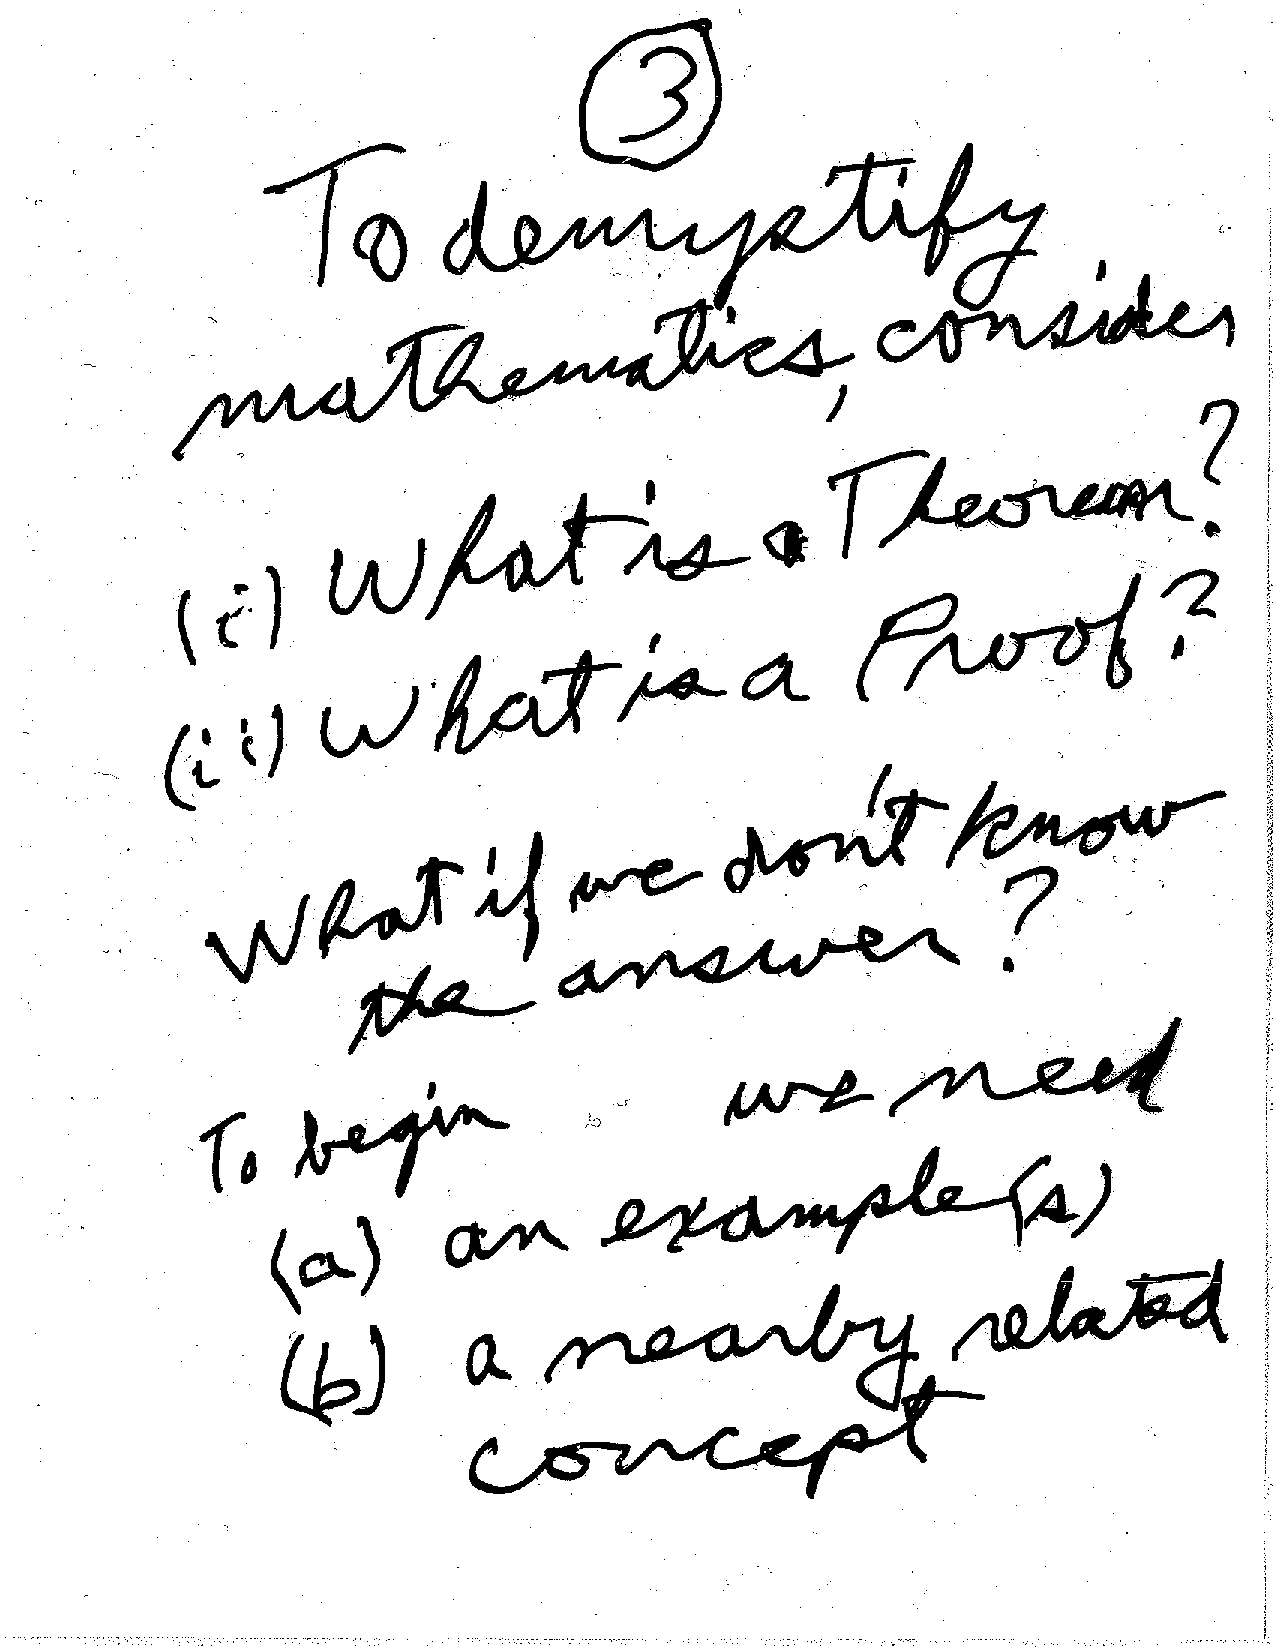
\includegraphics[scale=.5]{Pages/ST_3}

\newpage

Related Concept: Greek Syllogism

\underline{example:}
\begin{enumerate}
\item All men are mortal.
\item Socrates is a man.
\item Therefore, Socrates must die. 
\end{enumerate}

To analyze, recast in set theoretic terms via Venn Diagram.

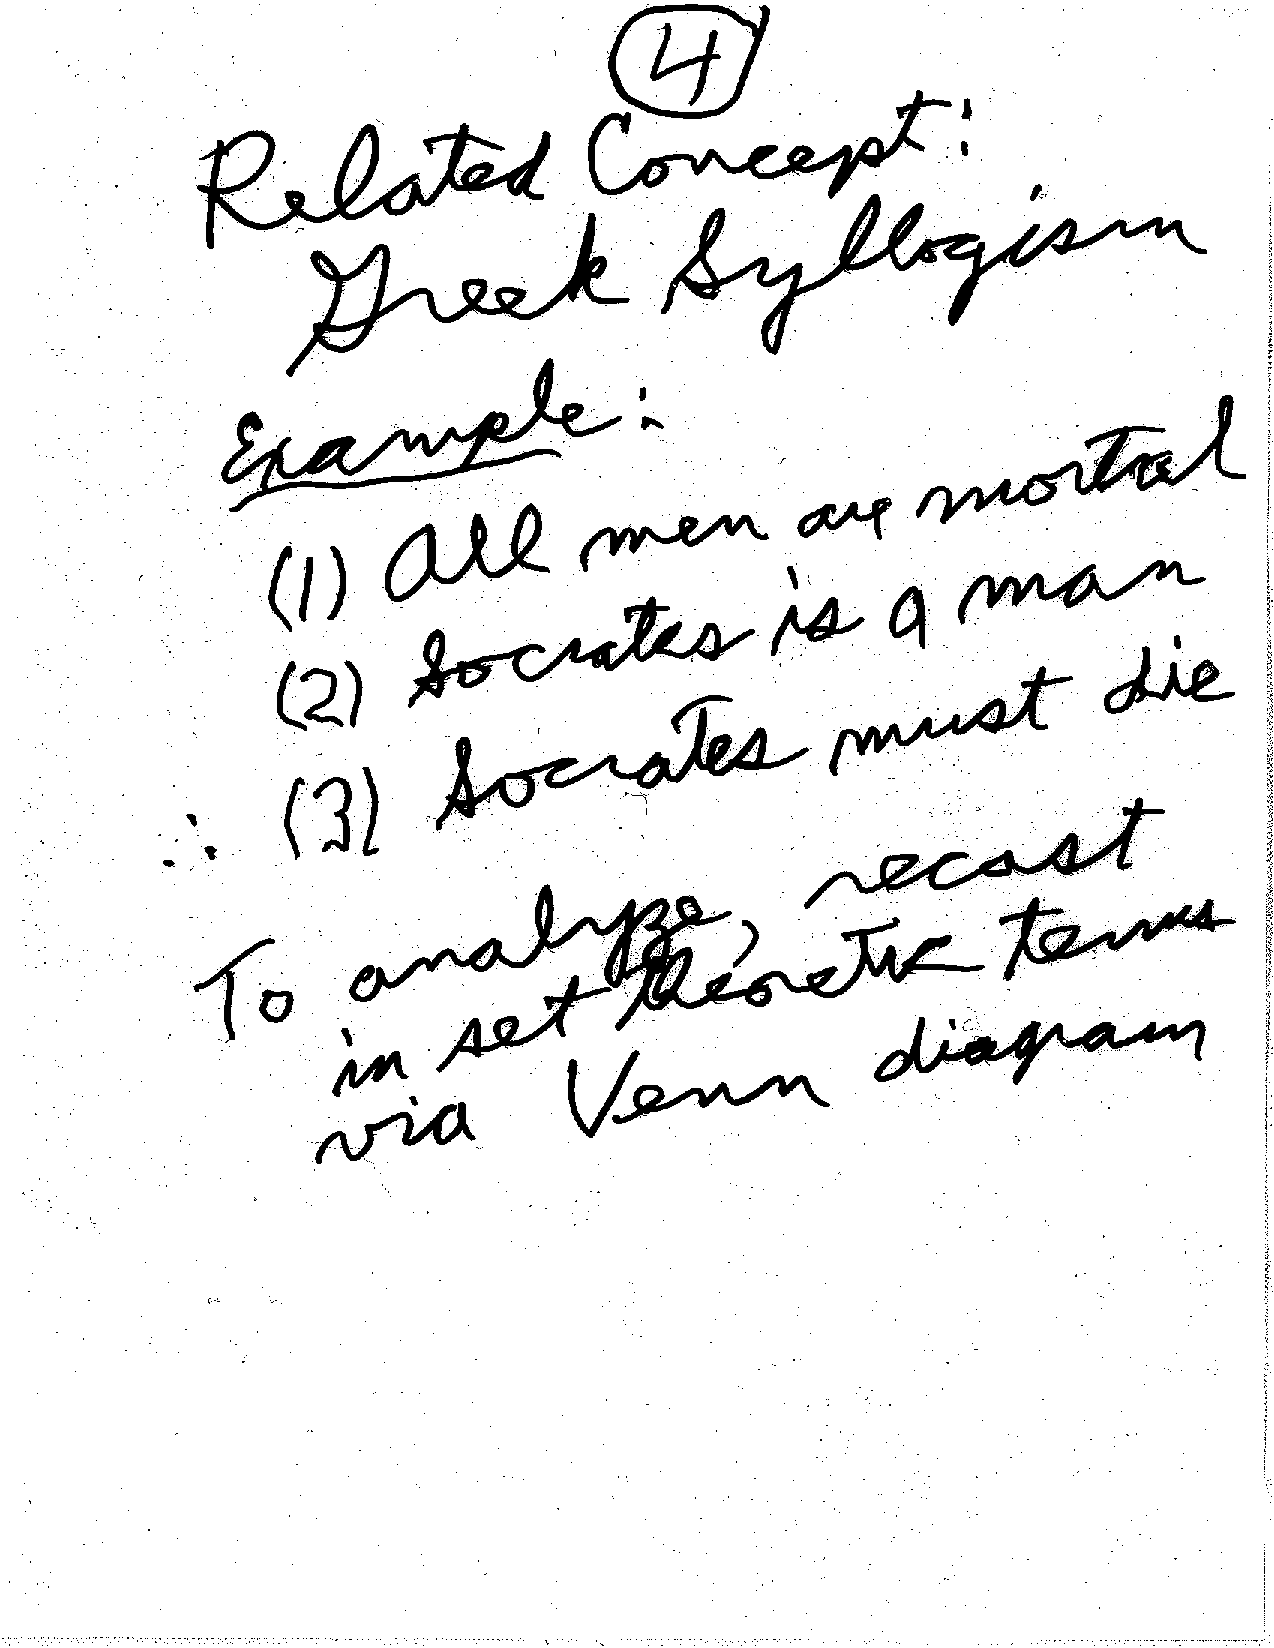
\includegraphics[scale=.5]{Pages/ST_4}

\newpage

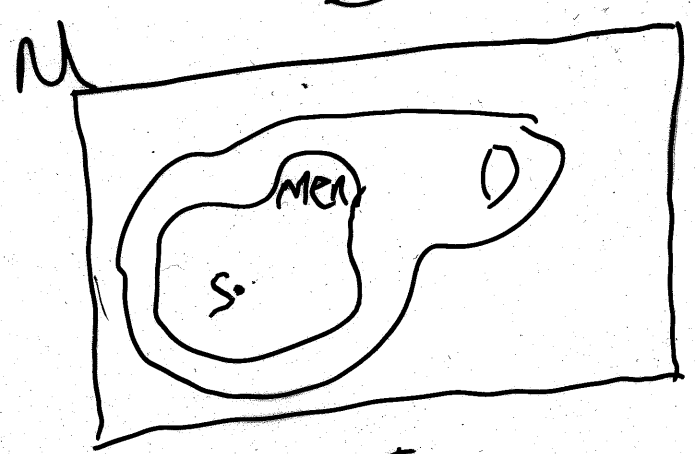
\includegraphics[scale=.2]{Pages/ST_5_im1}

$S$: Socrates\\
$M$: Set of Men\\
$D$: Things that will die\\
$\mathcal{U}$: Things on Earth

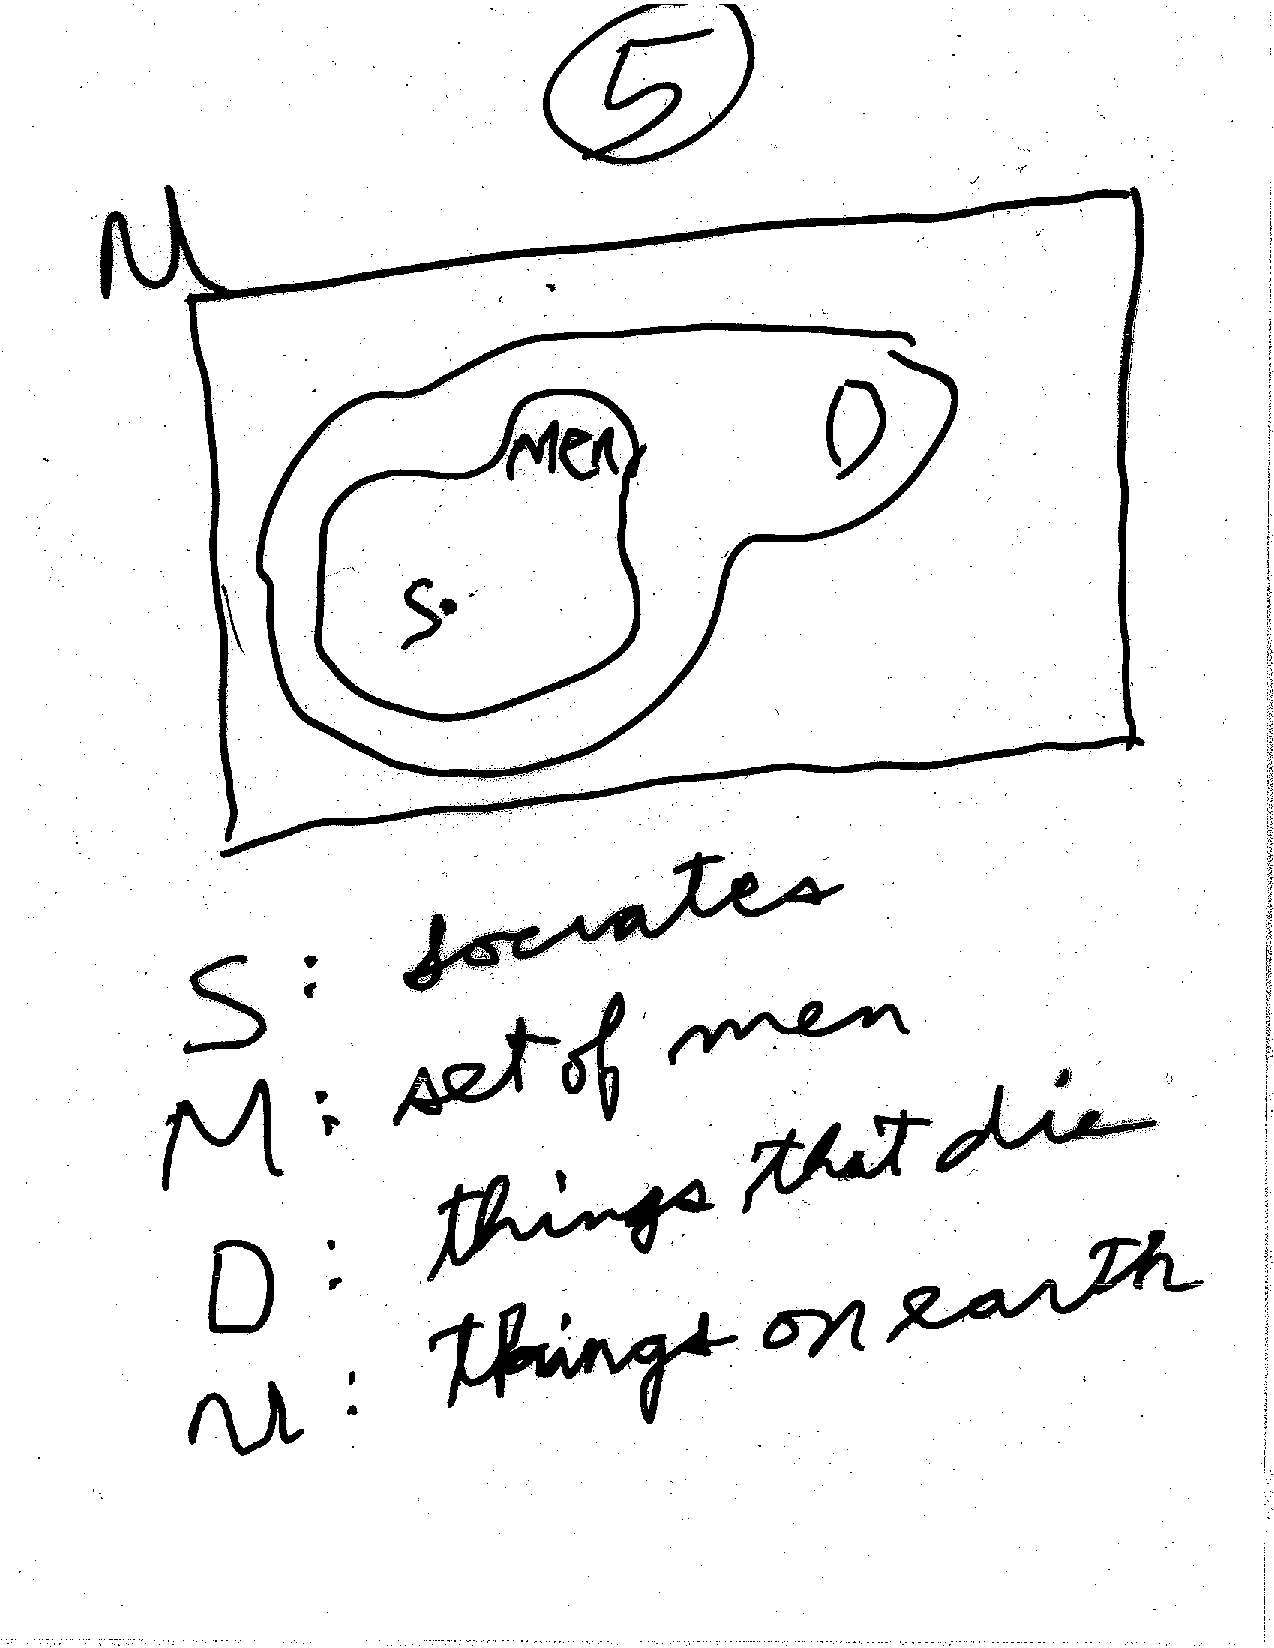
\includegraphics[scale=.5]{Pages/ST_5} 



%Zack: Pages 6,7,8,19,20

%Jack: 21, 9, 10, 11

%Koka: Pages 13, 13A, 22 ,22A, 22B


\section{Generate $\mathbb{N}$}


%Ruth: Pages L4A-L4G




\section{From $\mathbb{Z}$ to $\mathbb{R}$ via ordering}
%Jazz: ZR1-ZR5

%Kyler: ZR6 - ZR10

%Preethika: ZR11-ZR14


\section{Sequence and Limits}

%Aaron: First 2 pages and 48-50

%Hamza: 51-52B

\section{Limit and Convergence}

%Joe: 50-51

%Quinten: 52-53

%Farishta: 53A-54A

\section{Infinite Series}

%Sukhreet: IS1 - IS 7

%Matthew: IS8 - IS15

%Will: IS16 - IS23

%Rebecca: IS24 - IS32

\normalsize

\newpage

\noindent \underline{Theorem 2} (The Integral Test)
\vspace{5mm}
\\ Suppose $a_1 \geq a_2 \geq \cdots \geq 0$.
\\ Extend $a_n$ to $a(x)$ where $a(x)$ is continuous,
$a(n) = a_n$ and $a(x)$ decreases,
\\ Then $\sum_n a_n < \infty$ if and only if $\int_{1}^{\infty} a(x) dx < \infty$
\vspace{5mm}
\\ \underline{Proof}
$$\int_{1}^{\infty} a(x) dx = \sum_{n=1}^{\infty} \int_{n}^{n+1} a(x) dx$$
$$ \leq \sum_{n=1}^{\infty} \int_{n}^{n+1} a_n dx$$
$$ = \sum_{n=1}^{\infty} a_n $$

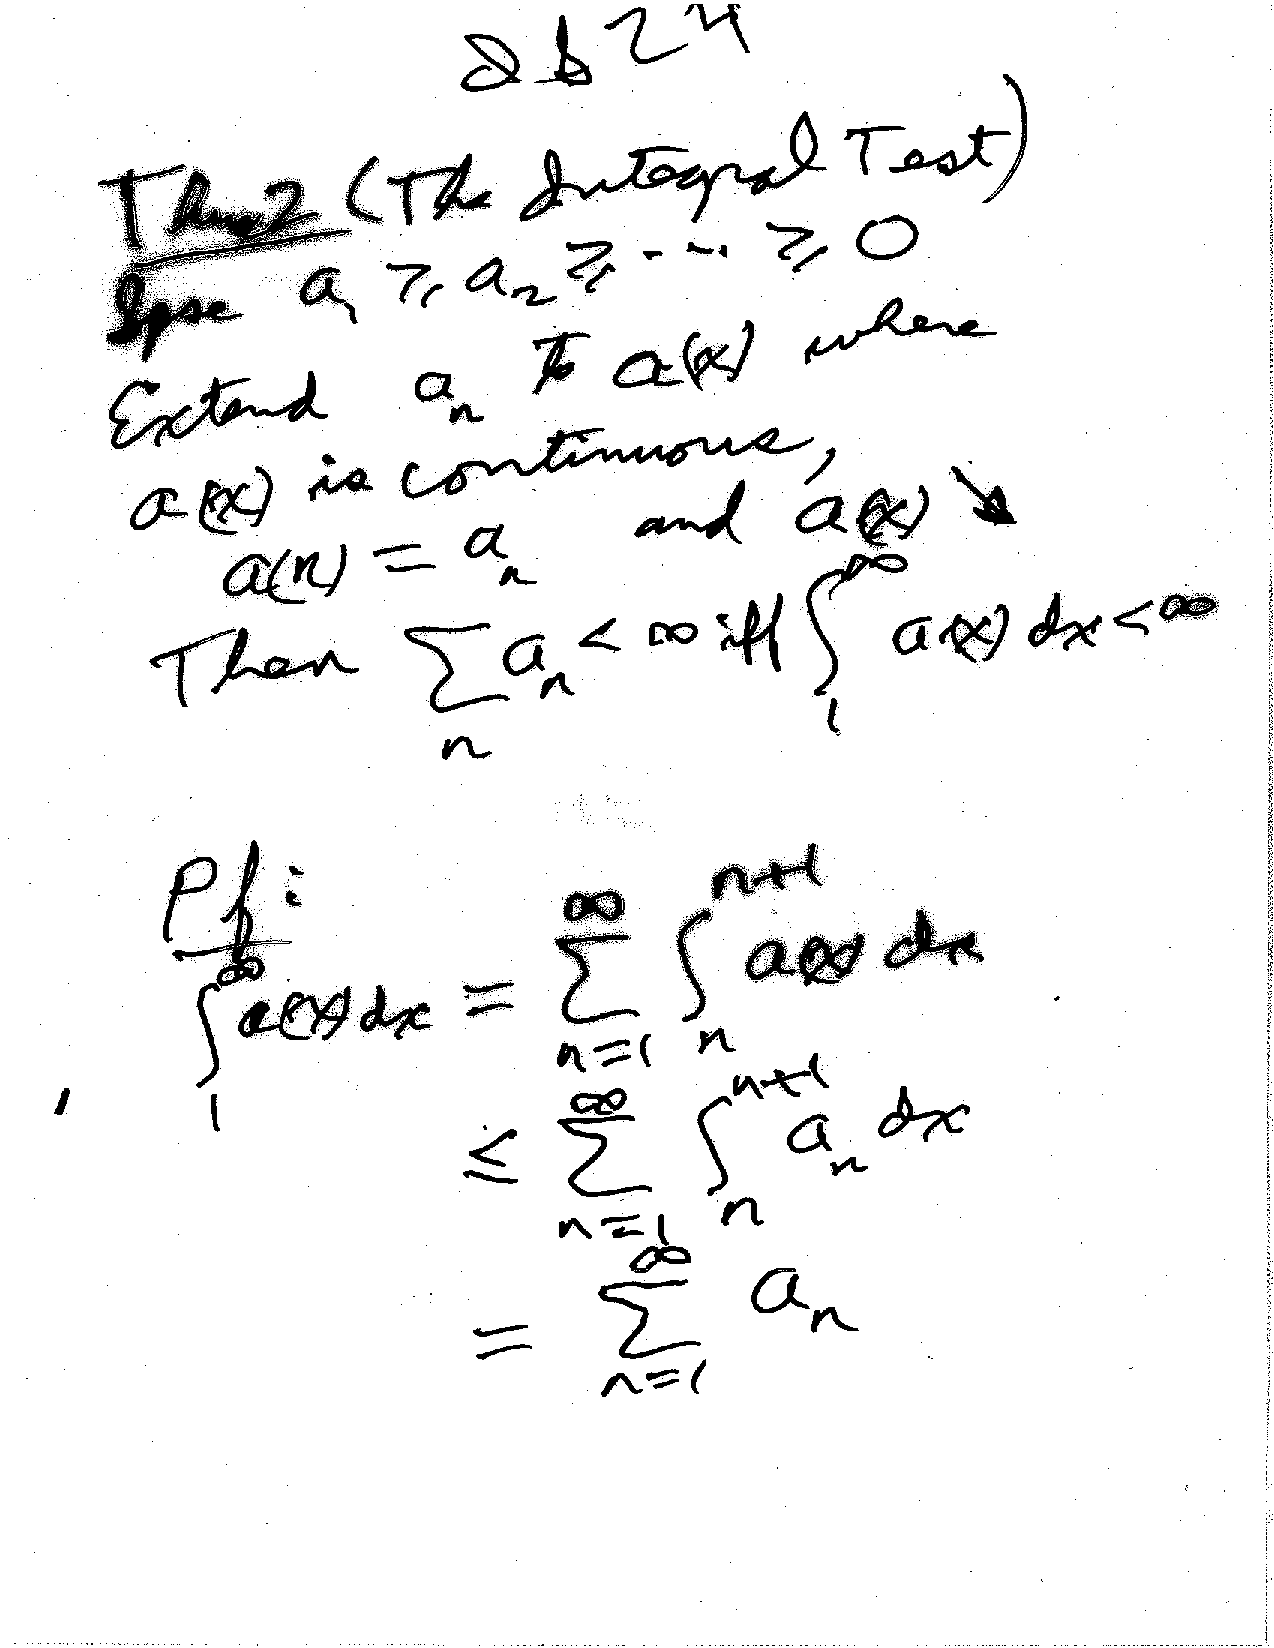
\includegraphics[scale=.5]{Pages/IS_24}

\newpage

\noindent Lower-bounding,

$$ \int_{1}^{n} a(x) dx = \sum_{n=2}^{\infty} \int_{n-1}^{n} a(x) dx$$
$$ \geq \sum_{n=2}^{\infty} \int_{n-1}^{\infty} a_n dx $$
$$ = \sum_{n=2}^{\infty} a_n$$

\noindent Hence, $\sum_{n=2}^{\infty} a_n $ and $ \int_{1}^{\infty} a(x) dx$
\\ converge or diverge together.

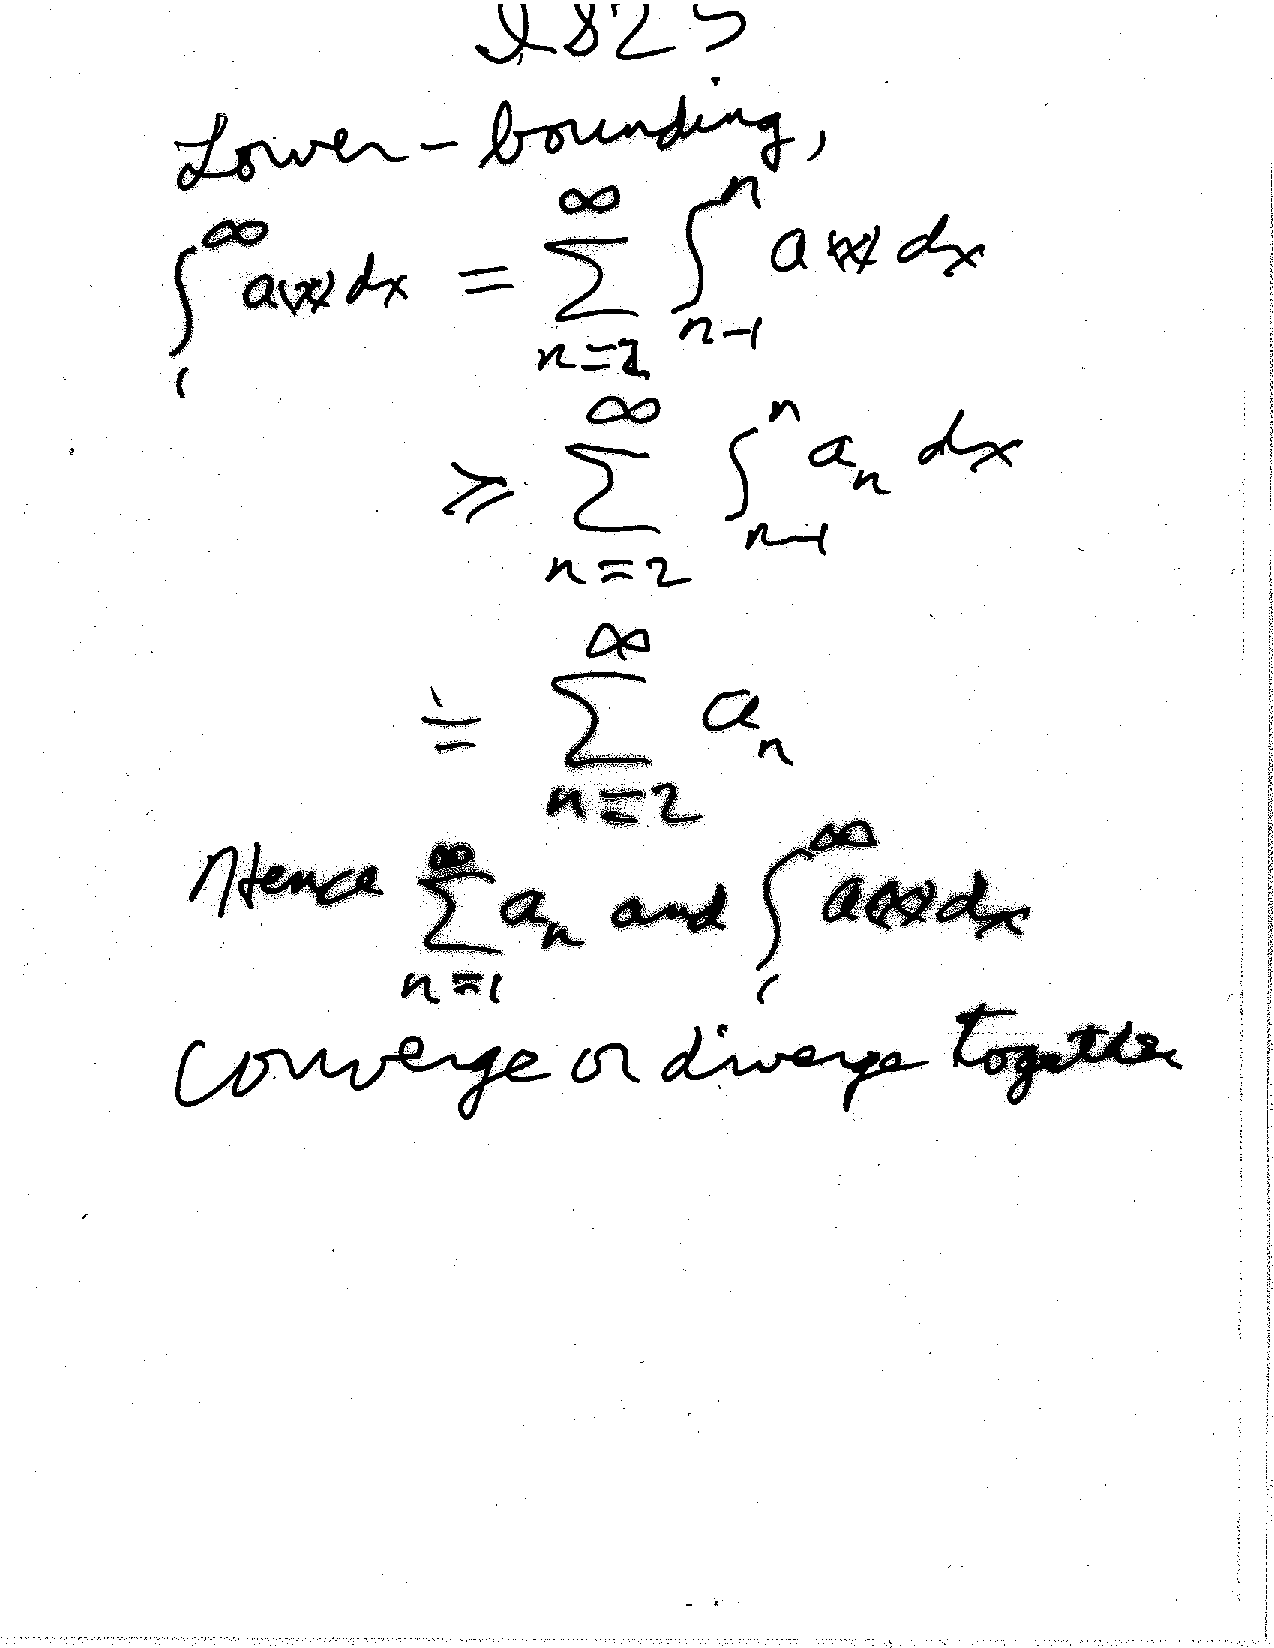
\includegraphics[scale=.5]{Pages/IS_25}

\newpage

\noindent Are $\sum_{j=1}^{\infty} a_j$ and $ \sum_{k=1}^{\infty} b_k$ equal, where 
\\$$b_k = \sum_{n_k \leq j \leq n_{k+1}} a_j$$
and $n_o = 0 < 1 = n_1 < n_2 < \cdots $? 
\\ \vspace{2mm}

\noindent More generally, when do all re-orderings of the terms of a series produce the same sum?

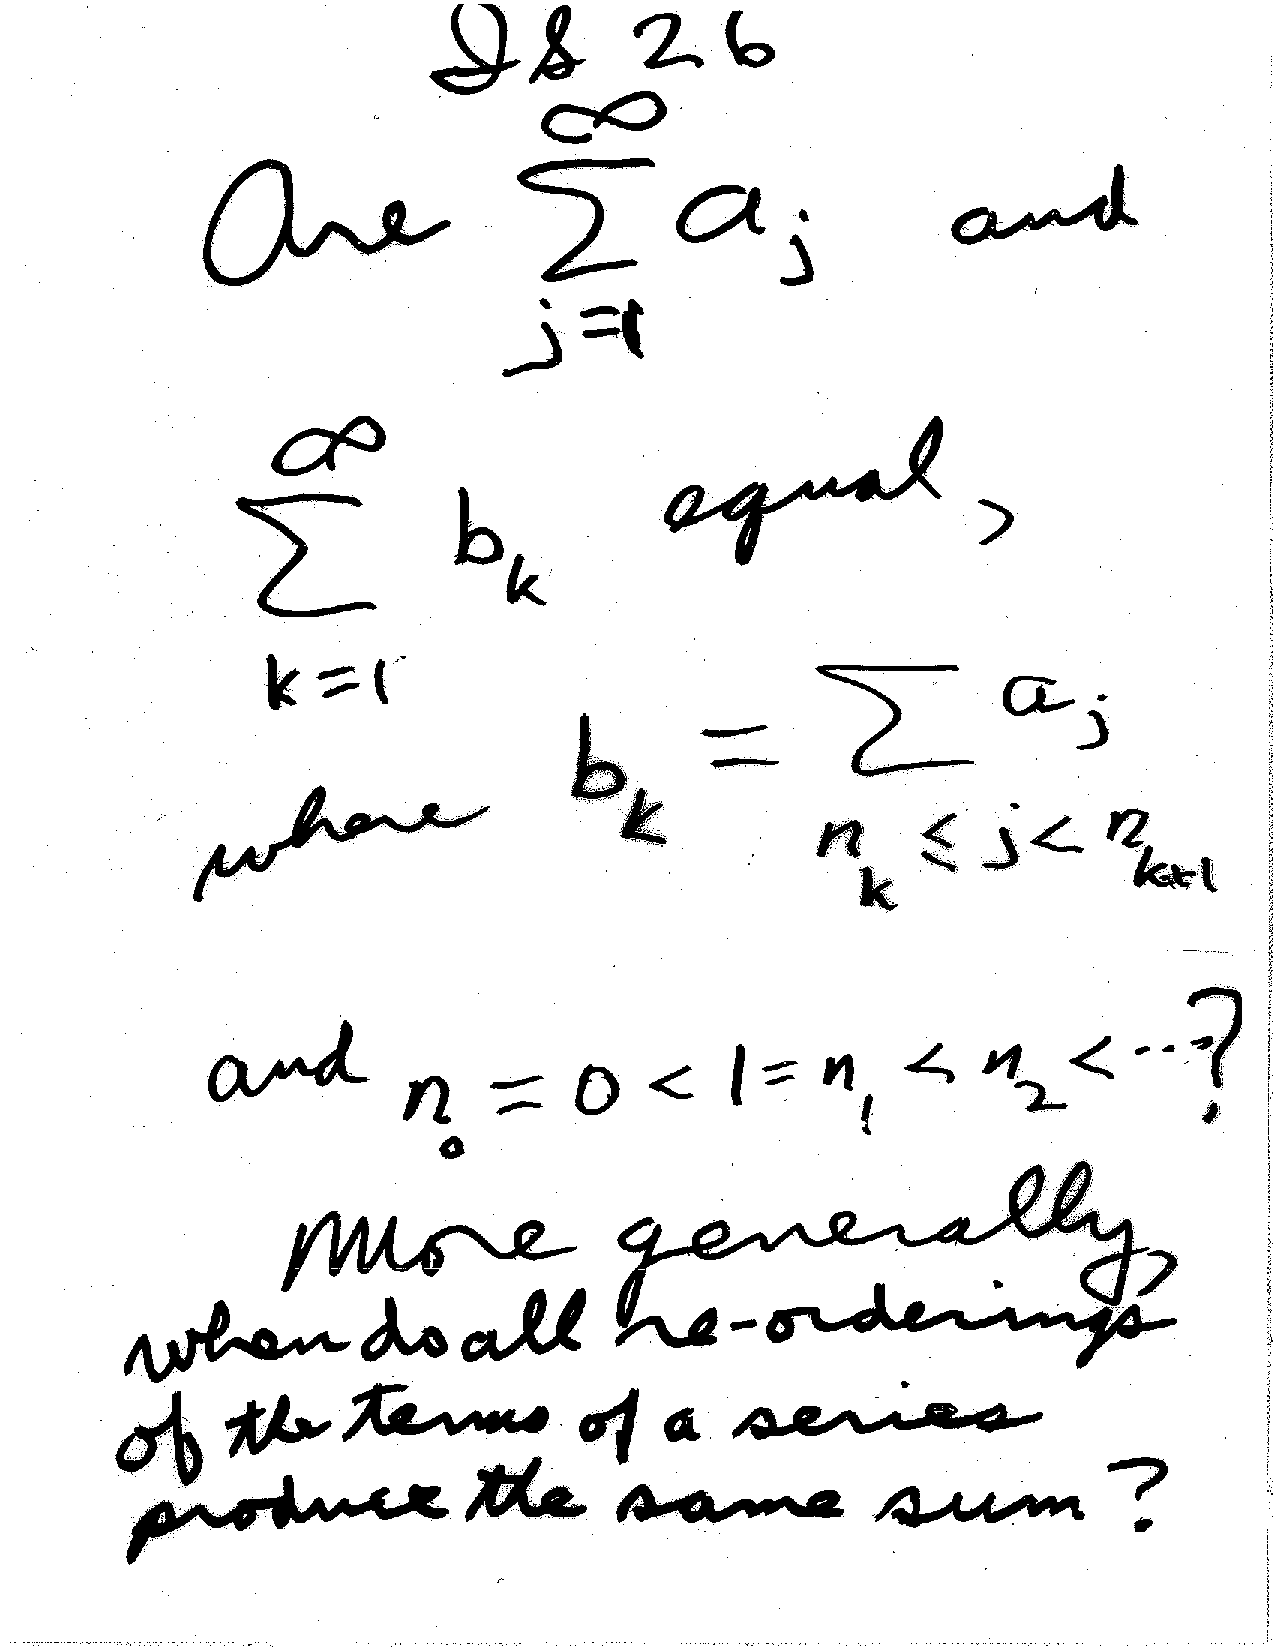
\includegraphics[scale=.5]{Pages/IS_26}

\newpage

\noindent \underline{Theorem:} Let $a_j \geq 0$
\\ and $F_1 \subseteq F_2 \subseteq \cdots $ with
\\ $ \cup_{n=1}^{\infty} F_n = \mathbb{N} $ and $F_n$ is finite.
\\ Then $$\sum_{j=1}^{\infty} a_j = \lim_{n \rightarrow \infty} \sum_{j \in F_n} a_j$$
\vspace{5mm}
\\ \underline{Proof:} Take away
\\ $$ s < S_{\infty} \equiv \sum_{j=1}^{\infty} a_j$$
\\ $ \exists N < \infty$ such that for all 
\ $ n \geq N$, $a_1 + \cdots + a_n > s$

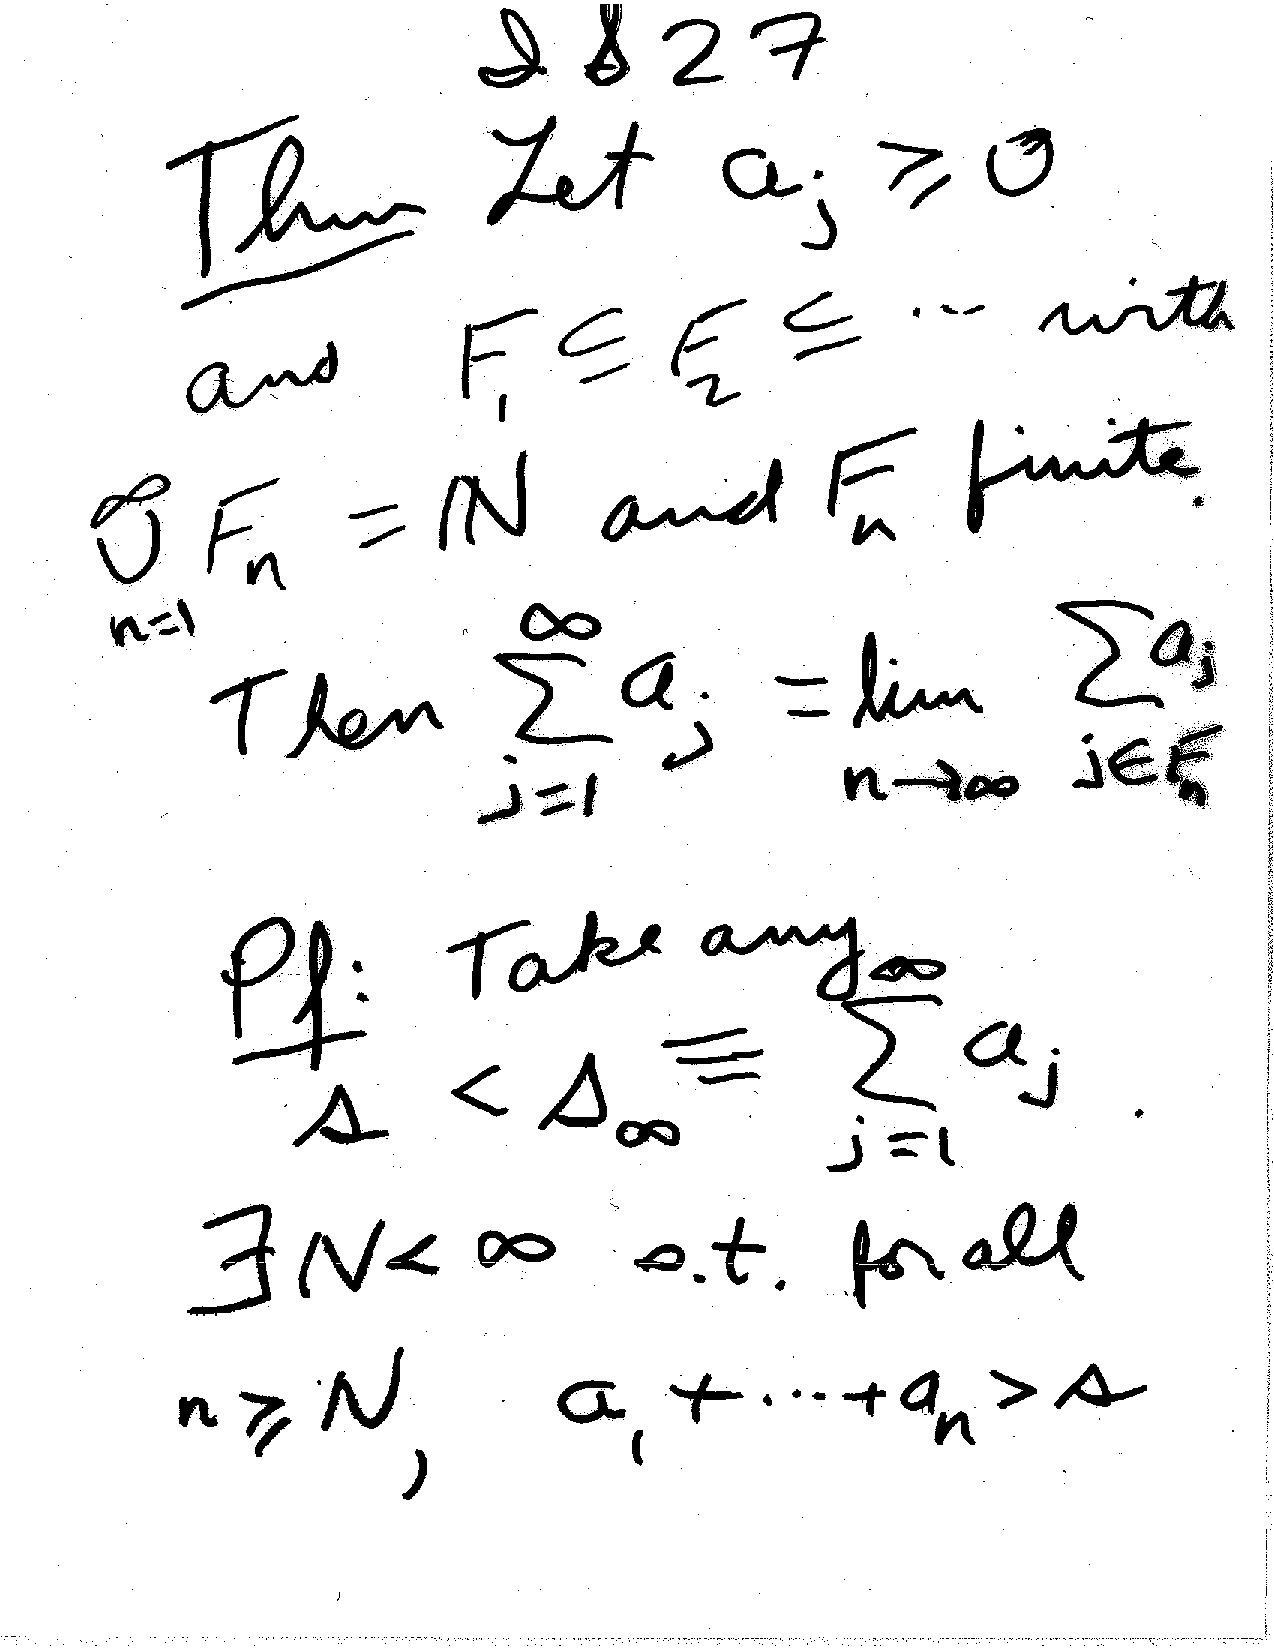
\includegraphics[scale=.5]{Pages/IS_27}

\newpage

\noindent Since $ \cup_{n=1}^{\infty} F_n = \mathbb{N}$, 
\\ $ \exists N' \geq N$ such that
\\ $\{1,2, \cdots, N\} \subseteq F_{N'}$ 
\\ Hence for all $ n \geq N'$
$$ \sum_{j \in F_n} a_j \geq \sum_{j=1}^{N} a_j > s $$
\\ \noindent Moreover, since $F_n$ is finite, 
$$\exists n* \geq max \{ j \in F_n \}$$
\\ Hence,$\sum_{ j \in F_n } a_j \leq \sum_{j=1}^{n} a_j \leq s_\infty $ \color{blue} TEXT CUT OFF \color{black}

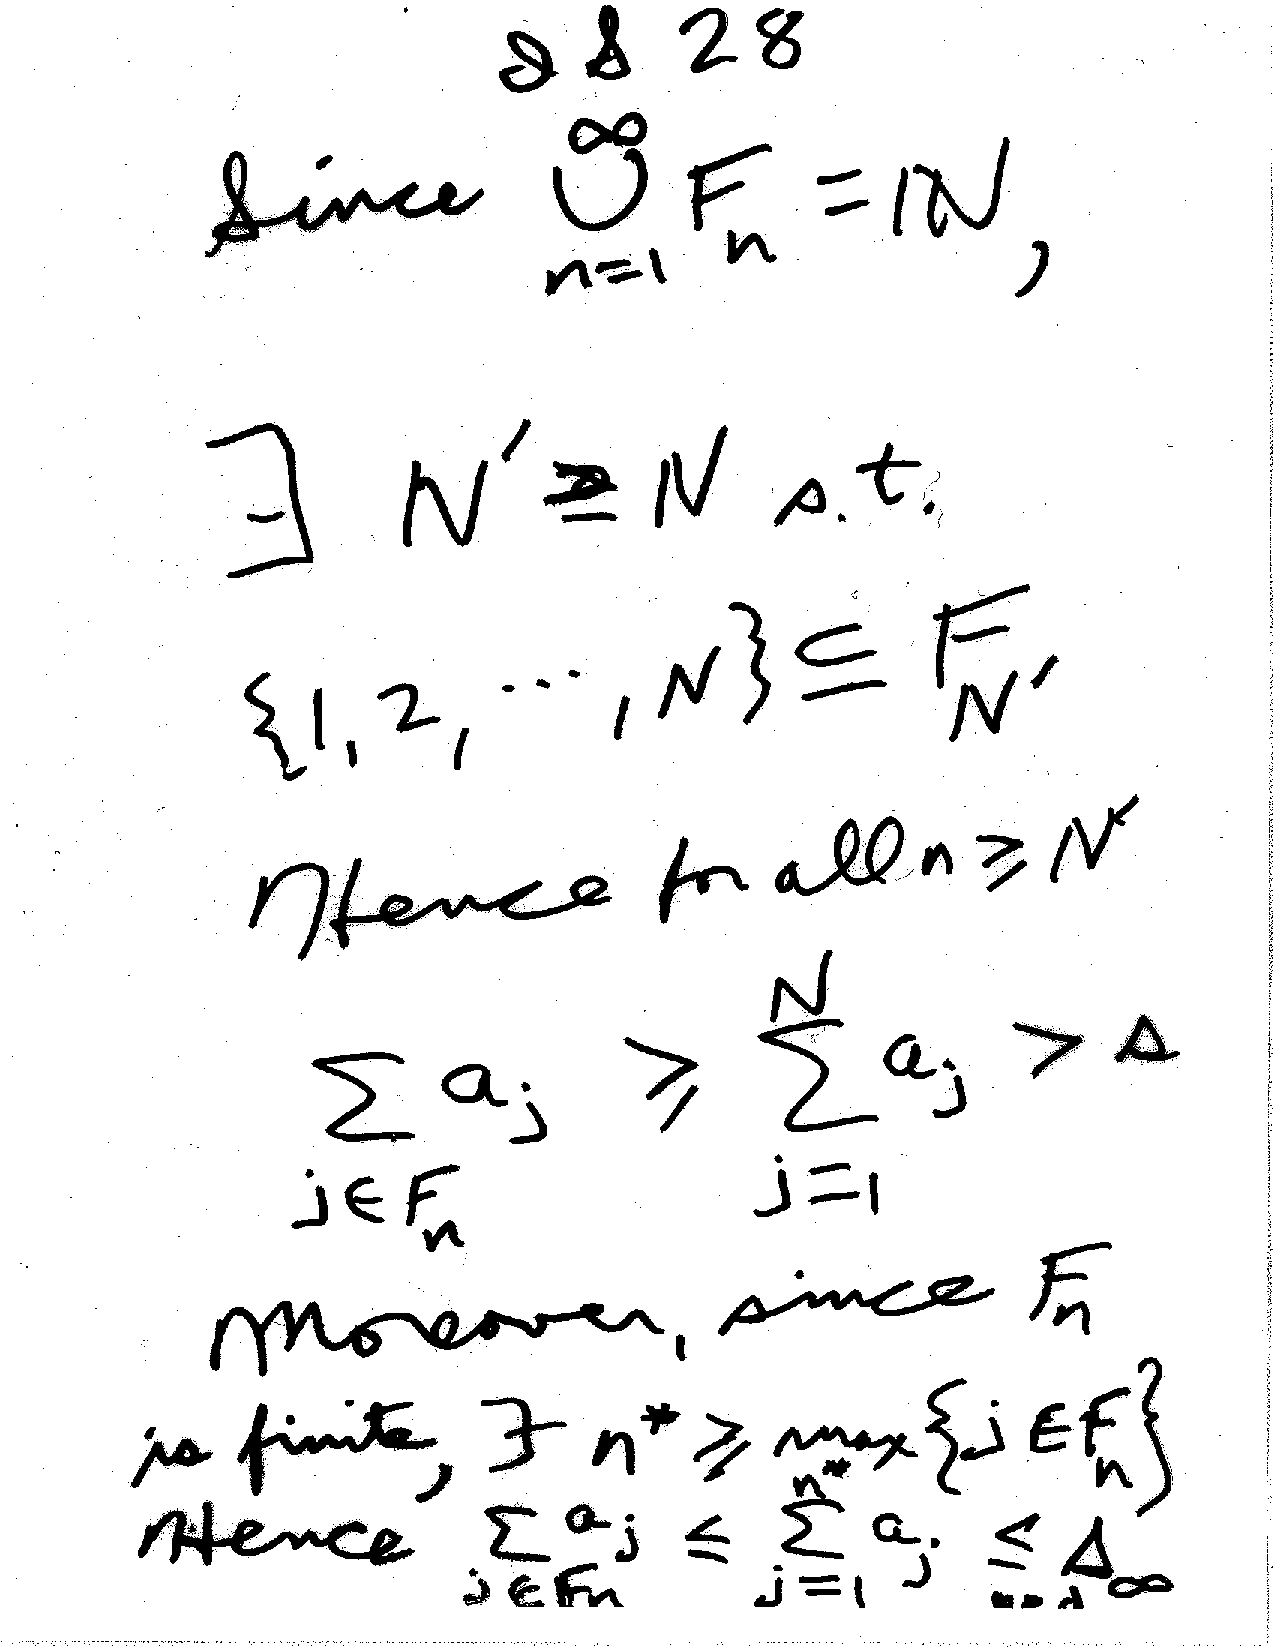
\includegraphics[scale=.5]{Pages/IS_28}

\newpage

\textbf{Summation by Parts}
\vspace{2mm}
\\ \noindent \underline{Theorem} Let $A_o = 0$, $A_n = a_1 + \cdots + a_n$ 
\\ Suppose $\{ A_n: n\geq 1\}$ is bounded.
\\ Let $b_1 \geq b_2 \geq \cdots $ with $b_n \rightarrow 0.$
\\ \noindent Then $\sum_{j=1}^{\infty} a_j b_j$ converges.

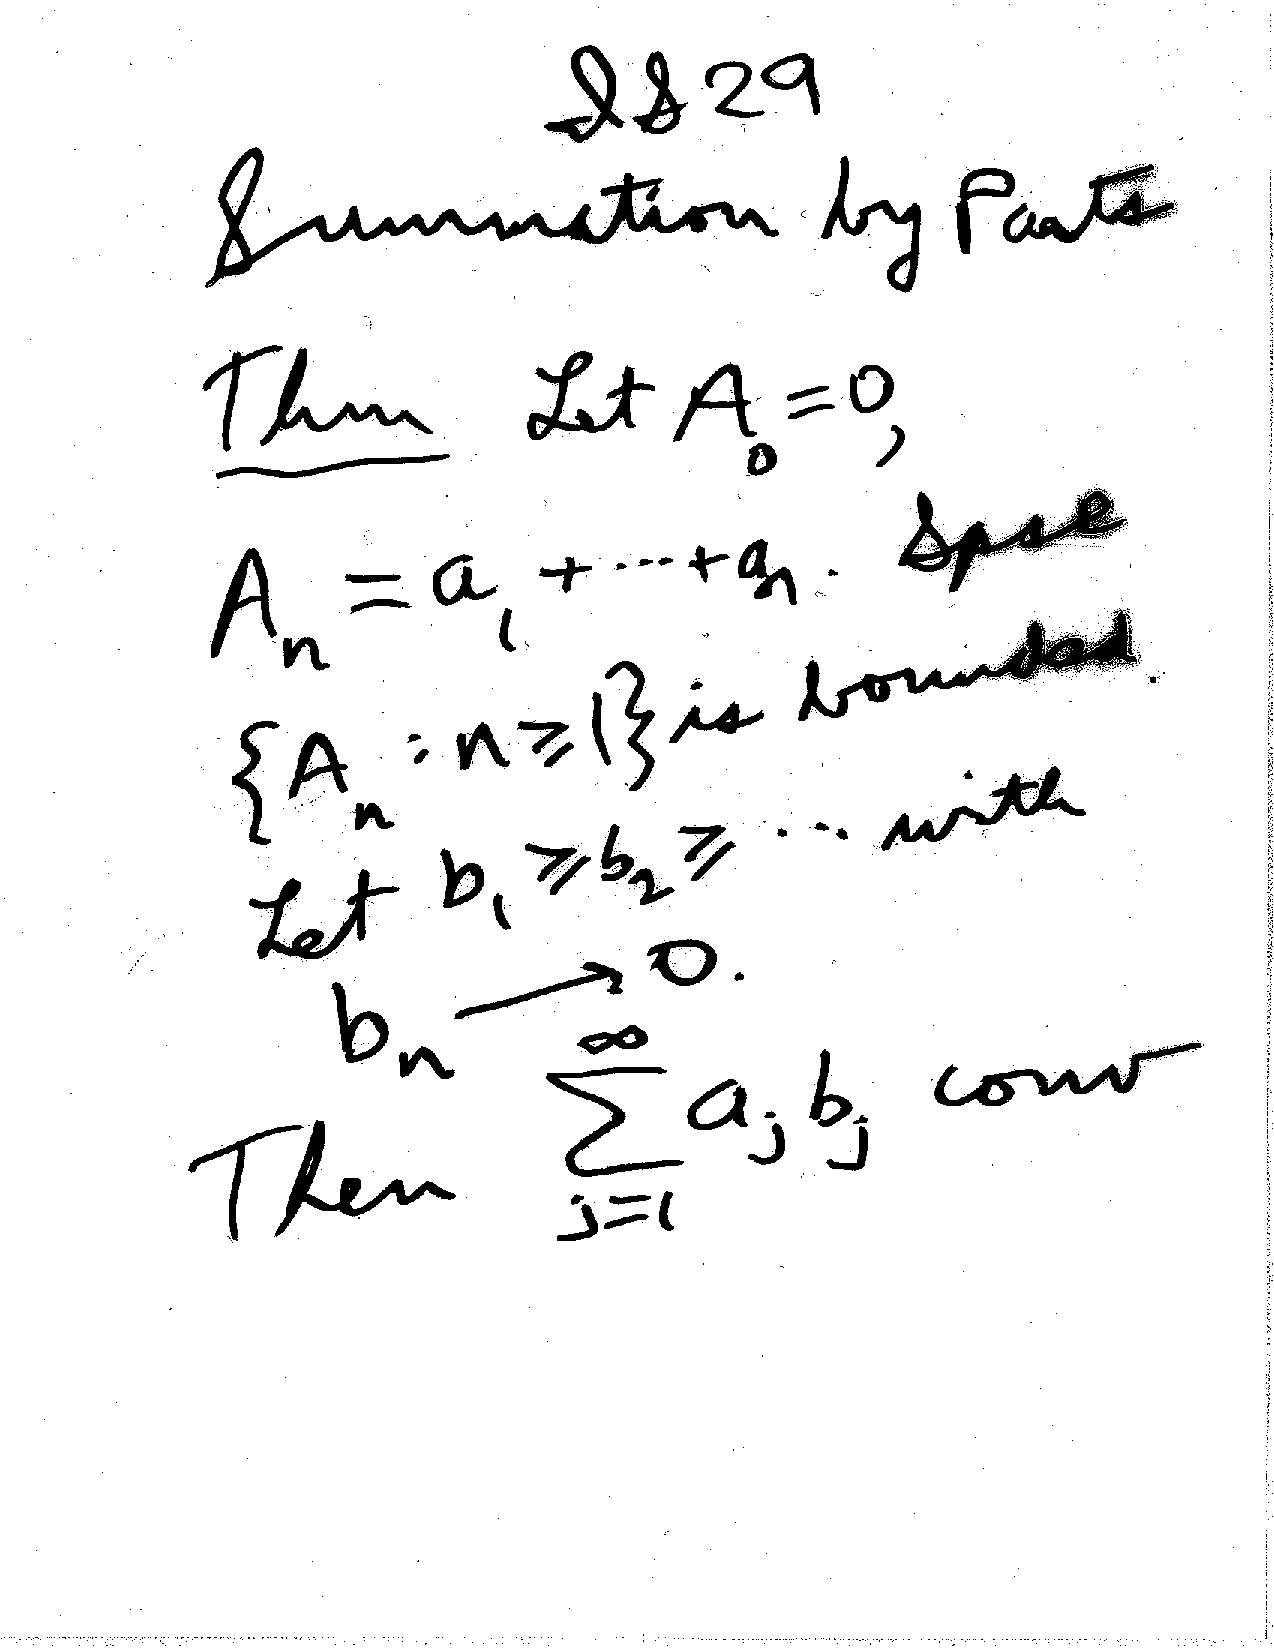
\includegraphics[scale=.5]{Pages/IS_29}

\newpage

\begin{center}
(for all $n\geq 1$)
\end{center}
\vspace{3mm}
\noindent \underline{Proof:} Suppose $|A_n| < A^* <\infty$.
\\Fix any $\epsilon > 0$. Take any $\delta > 0$ to be chosen later $\exists  N$ such that for $n\geq N$ $0 \leq b_n < \delta_\epsilon$
\\ For $n \geq N$ and $p \geq 0$,
$$ \sum_{j=n}^{n+p} A_j b_j = \sum_{j=n-1}^{n+p} (A_j - A_{j-1}) b_j$$ 
$$= \sum_{j=n}^{n+p} A_j b_j - \sum_{j=n-1}^{n+p-1} A_j b_{j+1}$$

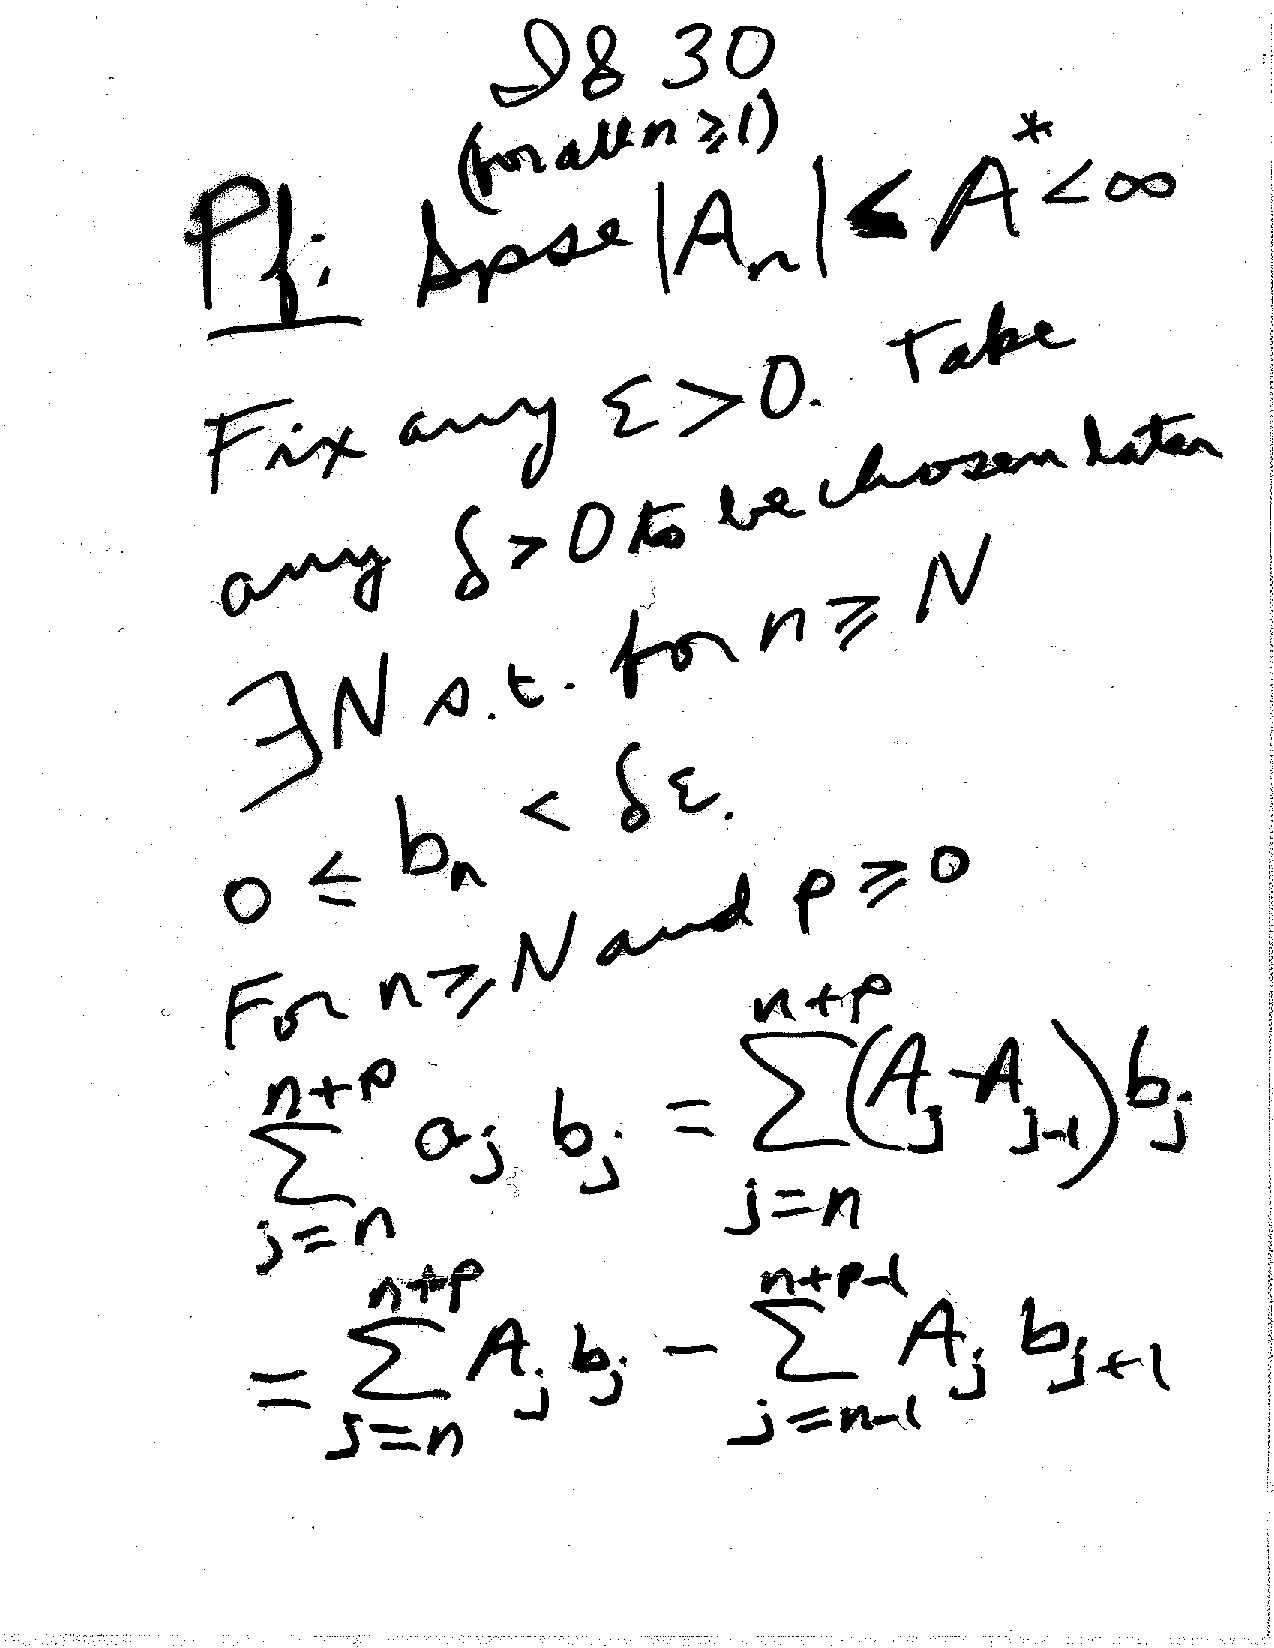
\includegraphics[scale=.5]{Pages/IS_30}

\newpage

\noindent So
$$|\sum_{j=n}^{n+p} a_j b_j|$$
$$ = |A_{n+p} b_{n+p} - A_{n-1} b_n + \sum_{j=n}^{n+p-1} A_j(b_j - b_{j+1})|$$
$$ \leq |A_{n+p}| b_{n+p} + |A_{n-1}| b_n + \sum_{j=n}^{n+p-1} |A_j| |b_j - b_{j+1}|$$

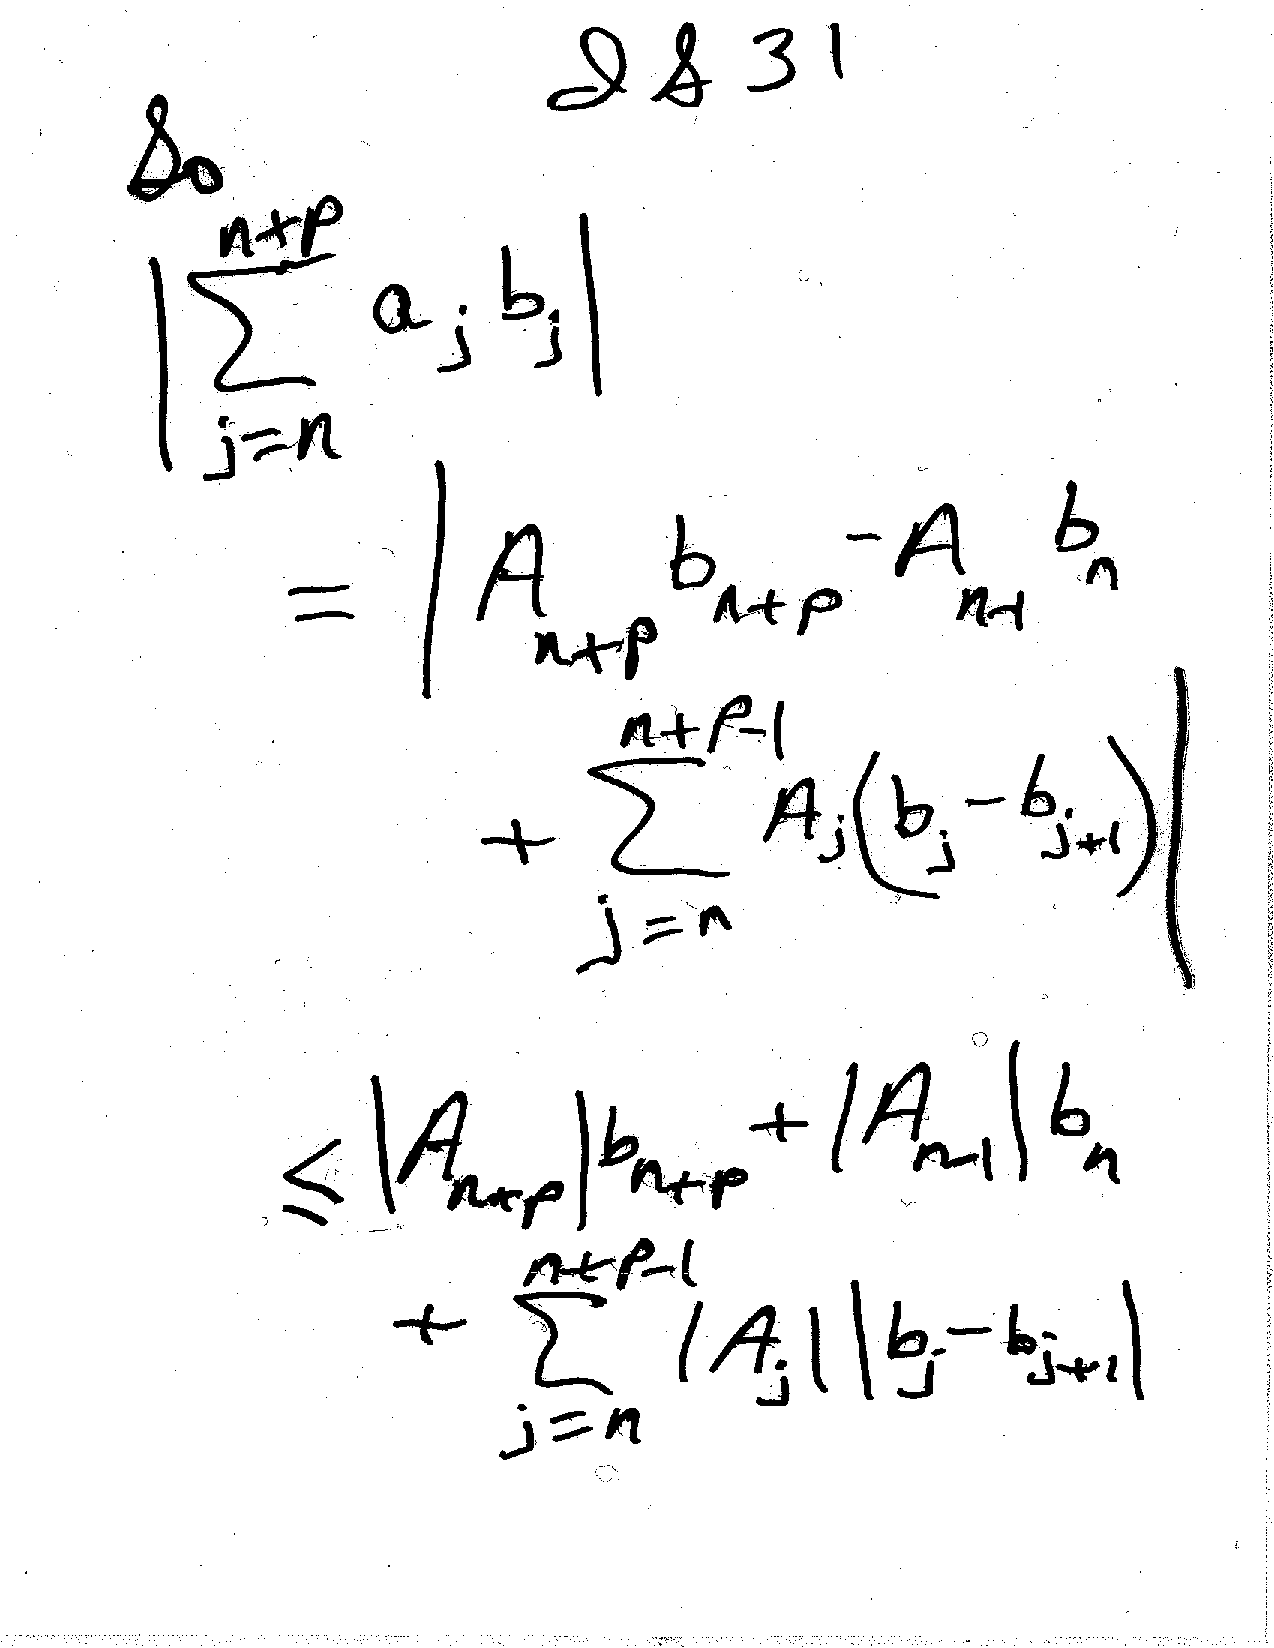
\includegraphics[scale=.5]{Pages/IS_31}

\newpage

$$\leq A^*\delta\epsilon + A^*\delta\epsilon + A^*\sum_{j=n}^{n+p-1} (b_j - b_{j+1})$$
$$ \leq 2A^*\delta\epsilon + A^*(b_n - b_{n+p})$$
$$ \leq 3A^*\delta\epsilon$$
\\ \noindent So let $\delta$ be any real number such that $0 < 3A^*\delta < 1$.
\\ \noindent Hence $\sum_{j=1}^n a_j b_j$ satisfies the Cauchy criterion. 
\\ Therefore, it converges.

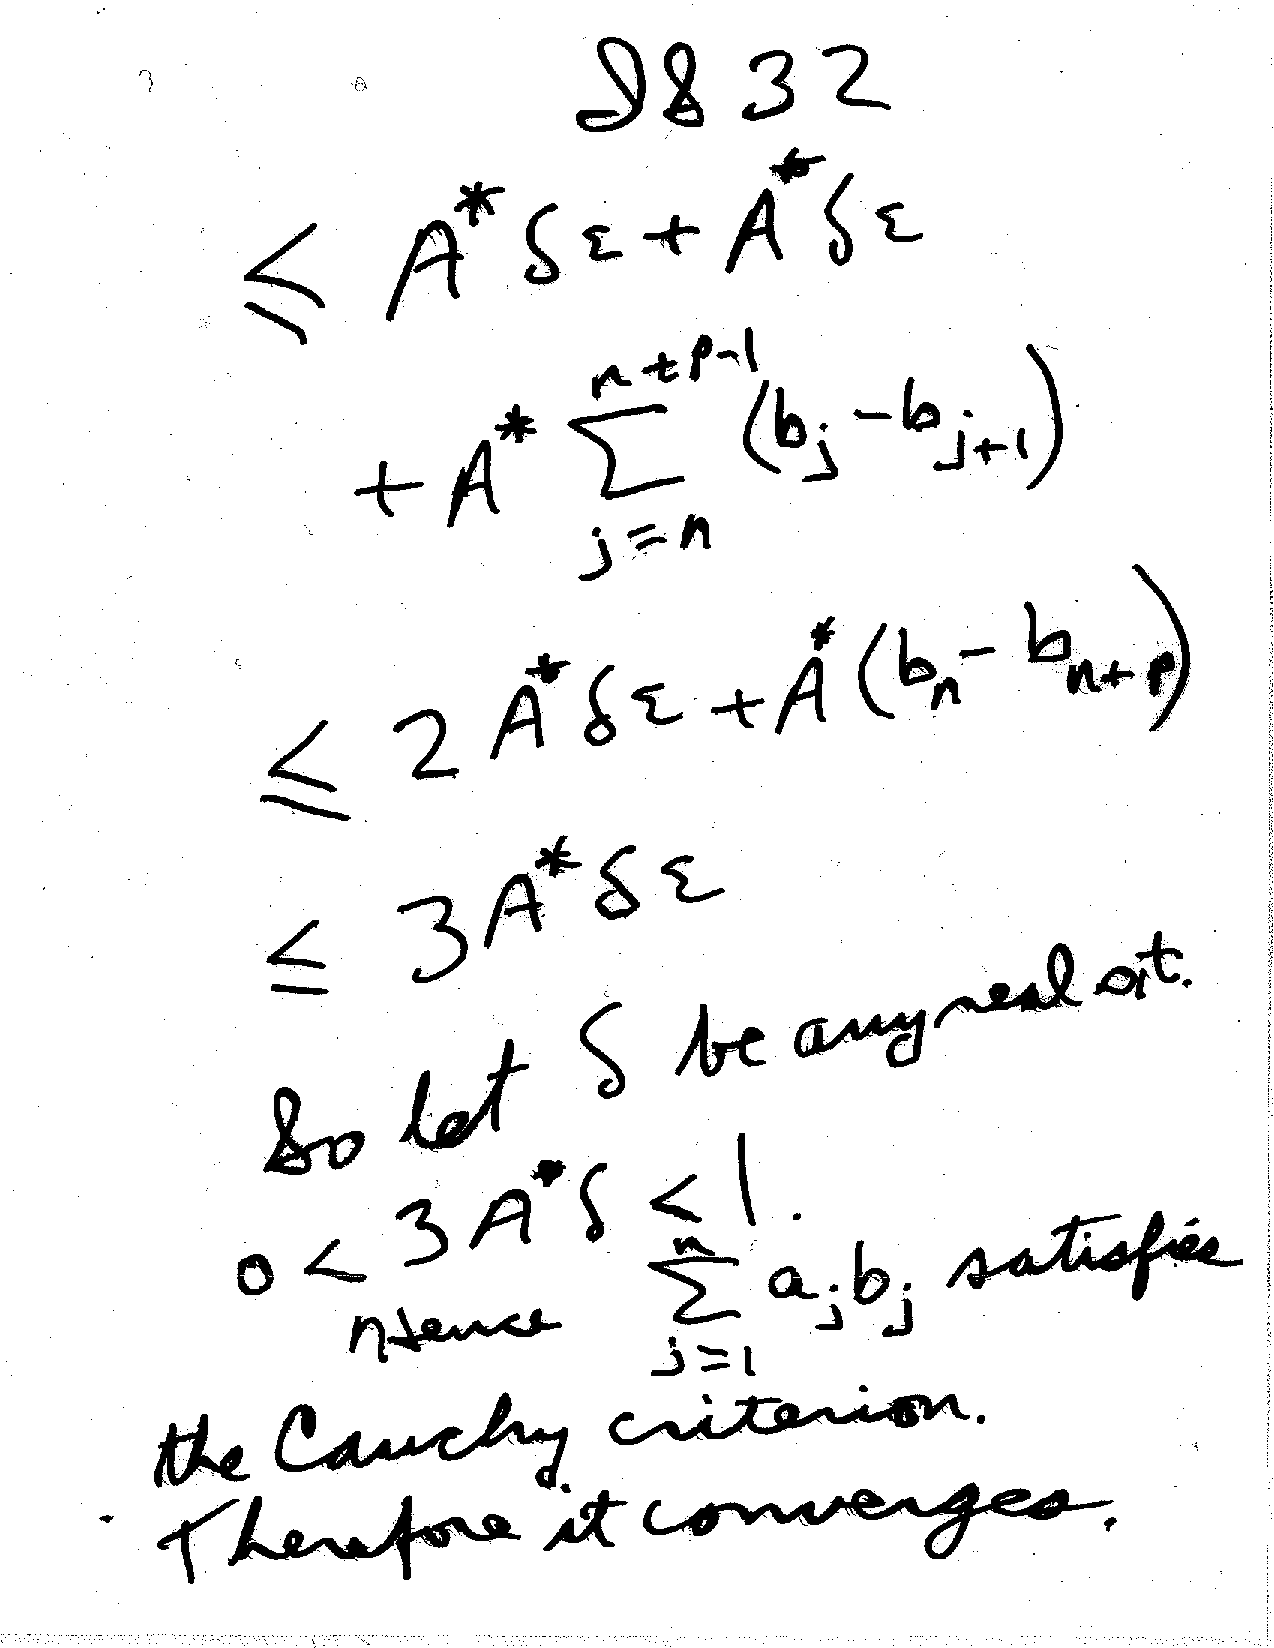
\includegraphics[scale=.5]{Pages/IS_32}

\newpage

\noindent 3) Thinking grandly, maybe all of mathematics can be put on a set theoretic foundation.\\ \indent Let's try to do so. 
\\ \vspace{2mm}
\hrulefill

\noindent \underline{Some Set Theory}
\vspace{2mm}
\\ \noindent A set can be defined by 
\begin{enumerate} [(i)]
\item listing its elements
\item listing the properties that determine membership in the set.
\end{enumerate}

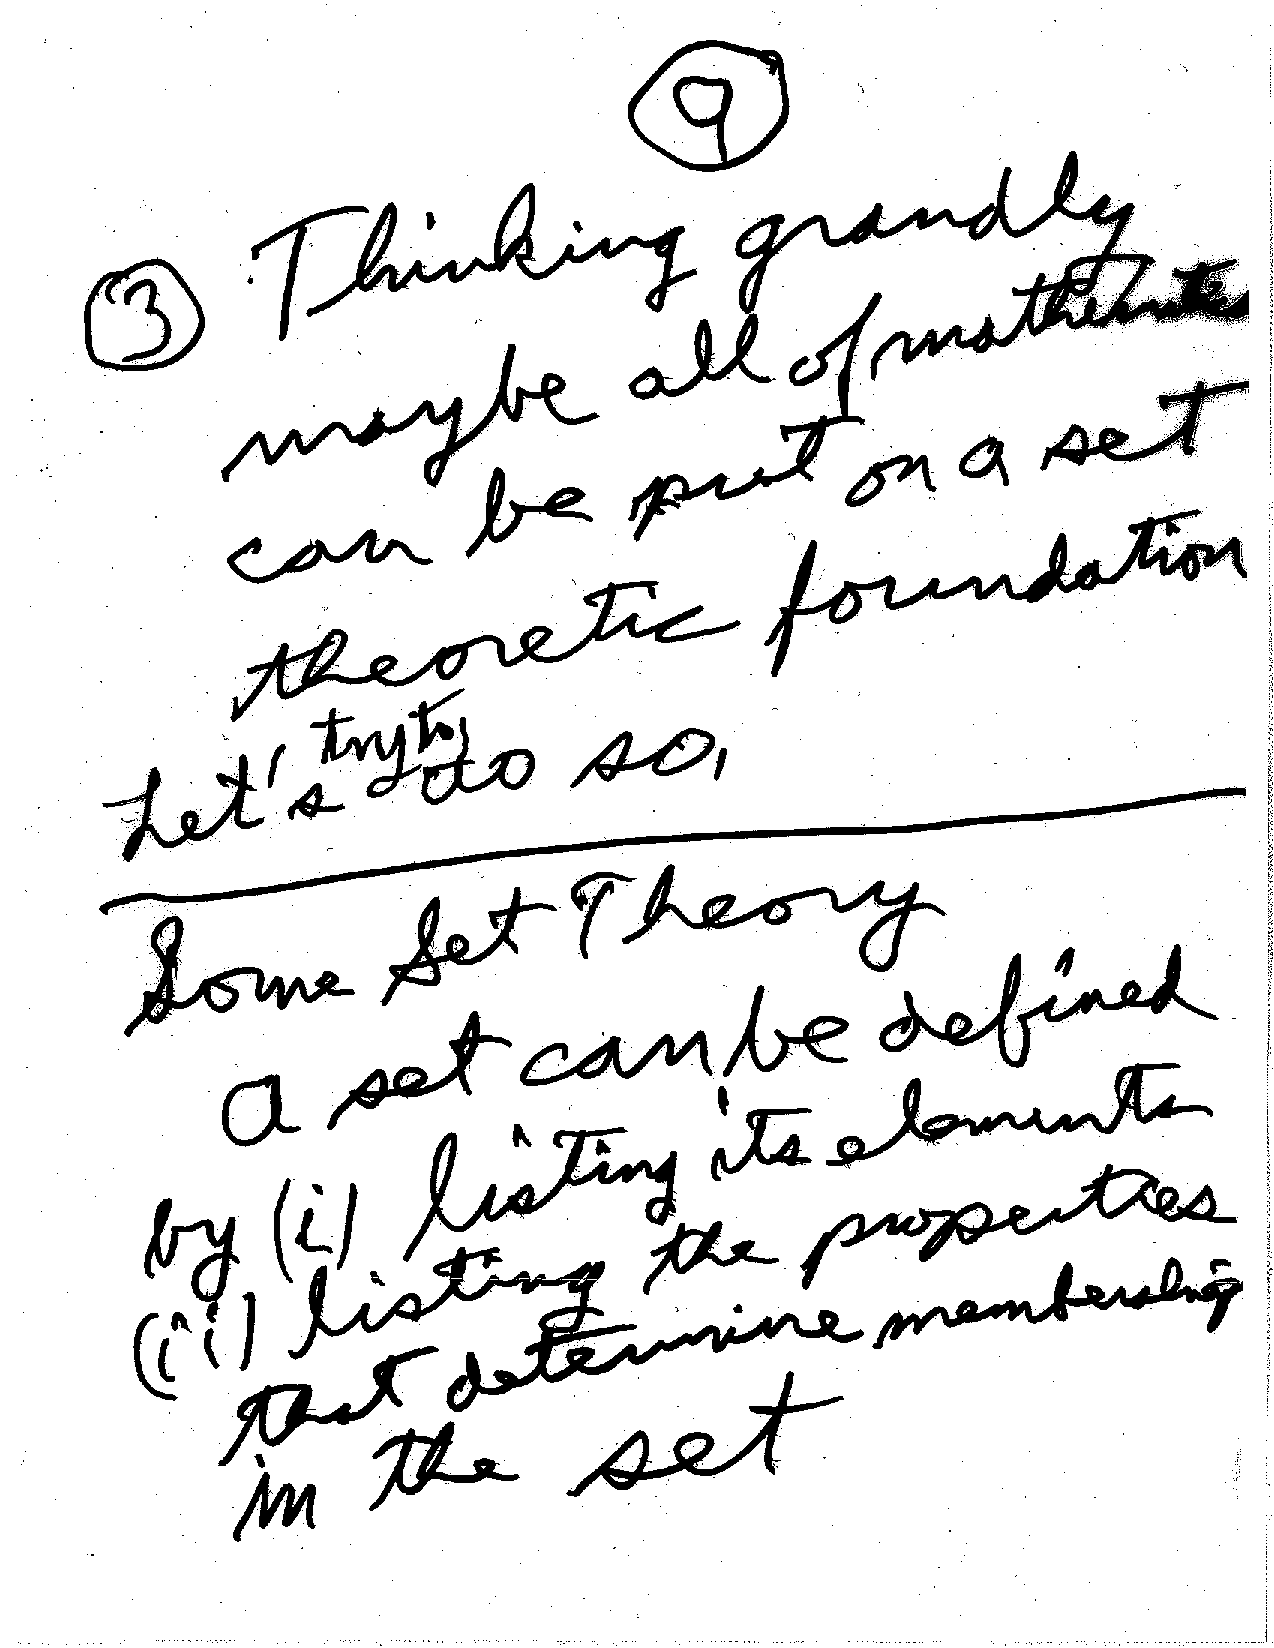
\includegraphics[scale=.5]{Pages/ST_9}

\newpage 

\noindent \underline{Examples}

\vspace{2mm}
\begin{itemize}
\item $\{1,2,5\}$ 
\item \{ cat, bat, dog\ \}
\item $\{\{1,2\},5\}$
\item \{ odd primes \}
\item \{ positive integers having no odd divisors \}
\end{itemize}

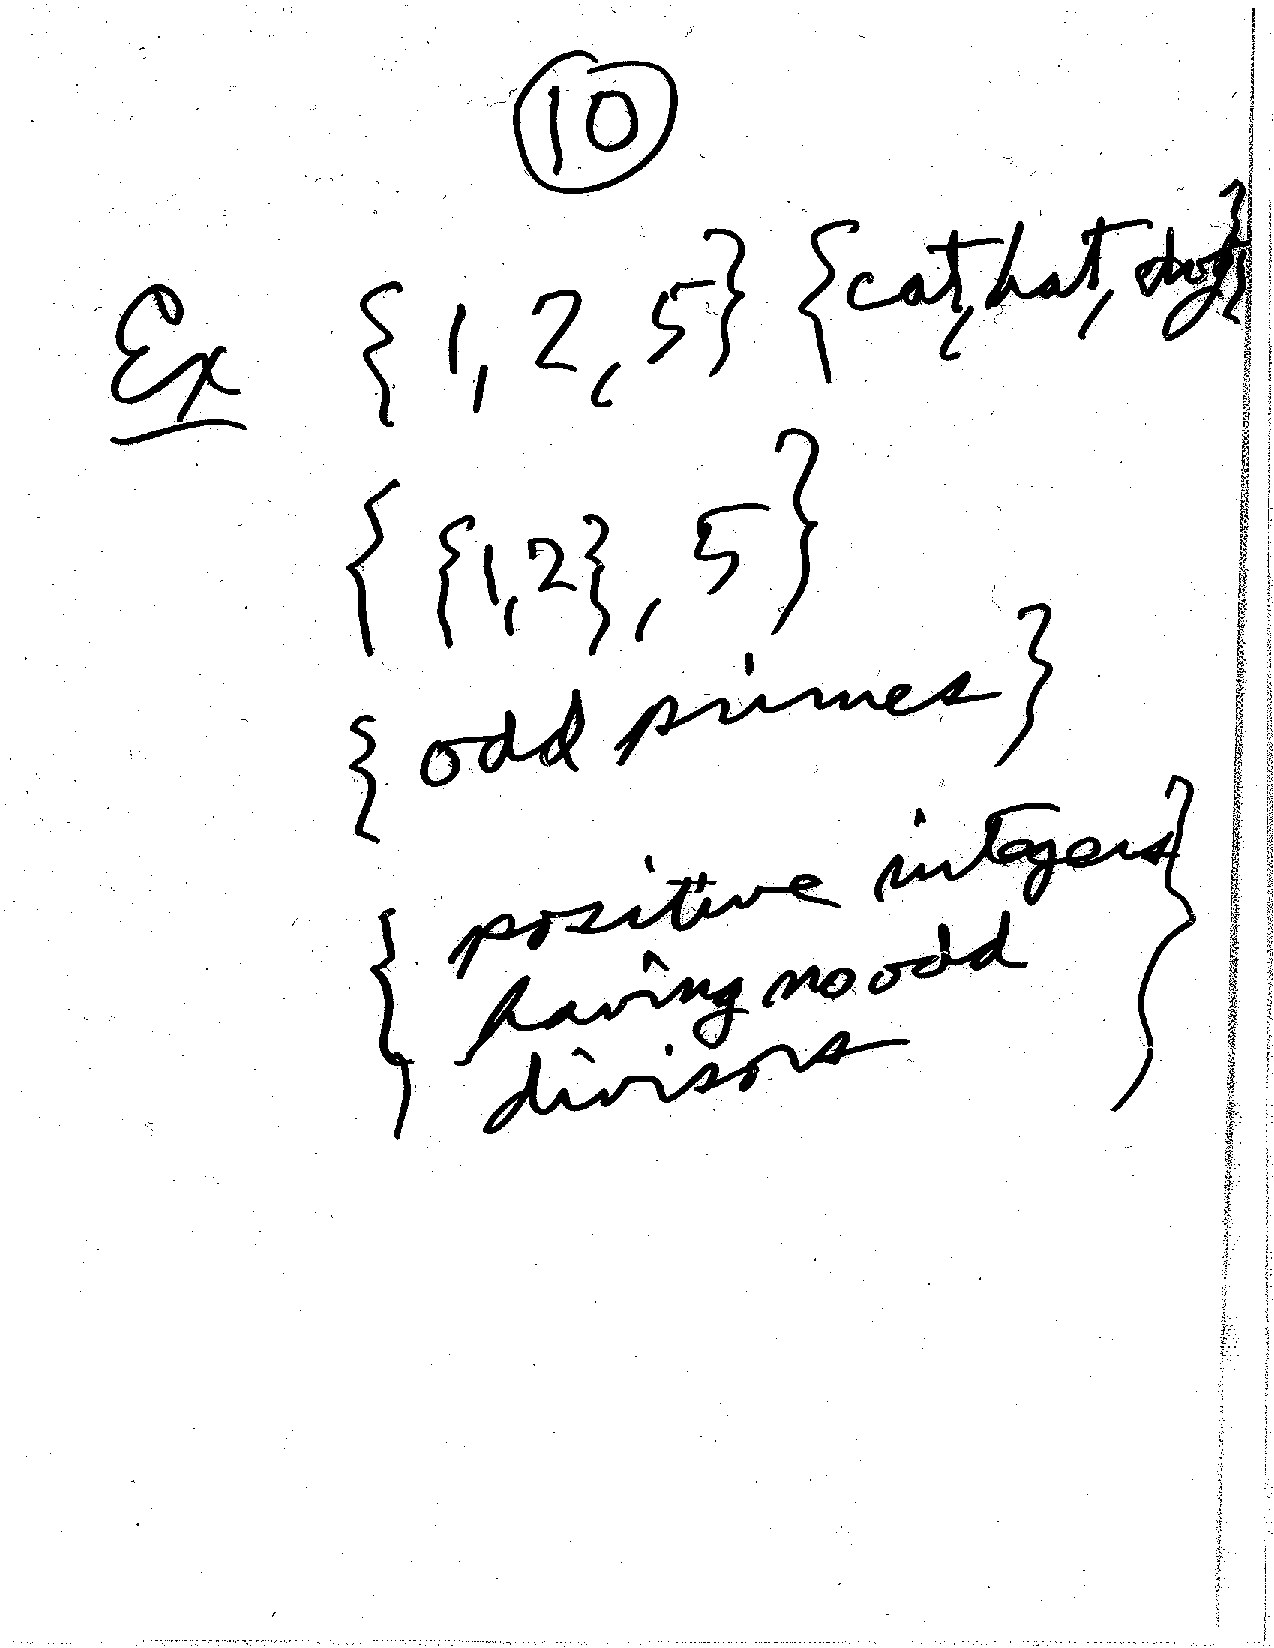
\includegraphics[scale=.5]{Pages/ST_10}

\newpage

\noindent How can we construct "new" sets from "old" sets?

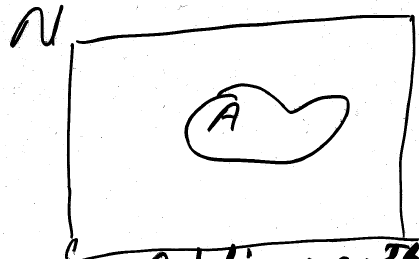
\includegraphics[scale=.5]{Pages/ST_11_im1}

\noindent Clearly, $A$ defines another set $$ A^c \equiv \{ x \in \mathbb{U}: x \notin A\} $$

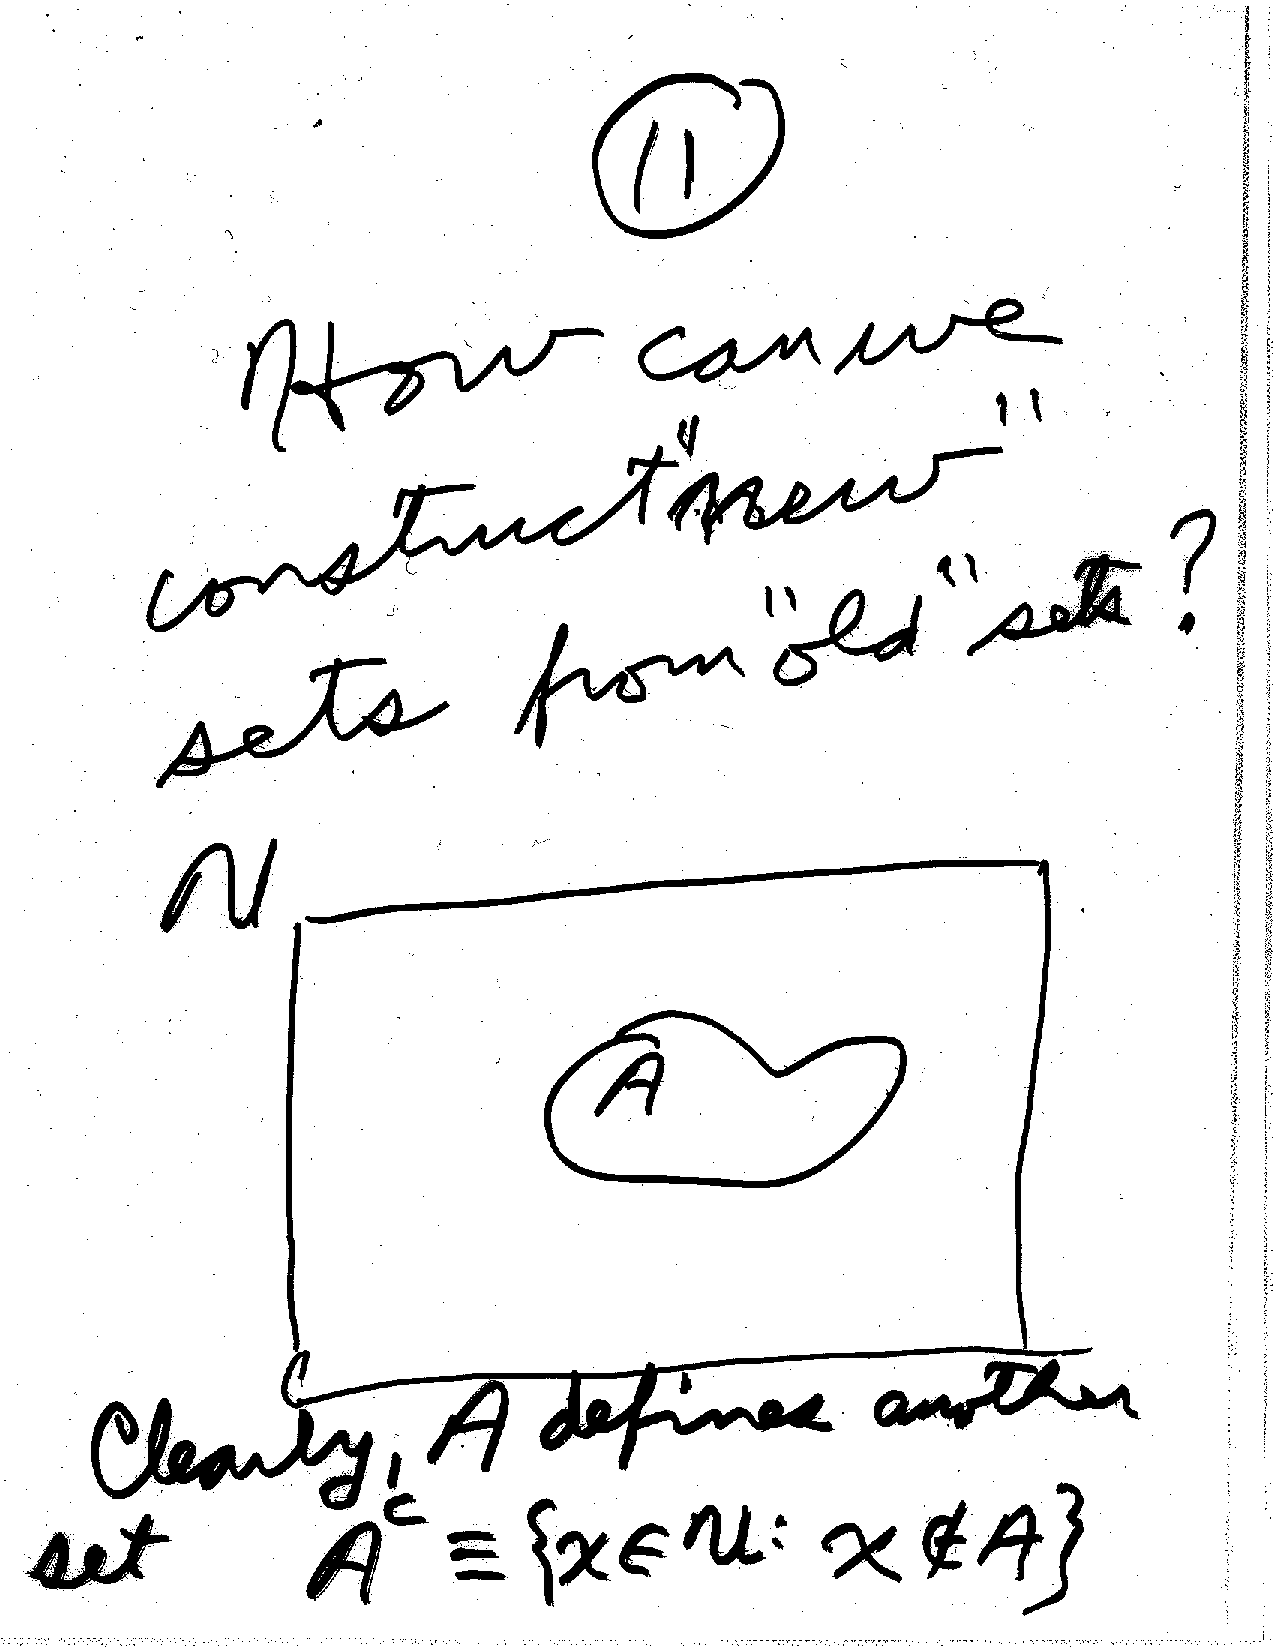
\includegraphics[scale=.5]{Pages/ST_11}

\newpage

\noindent So: What is a THEOREM?
\vspace{2mm}
\\ \noindent It always has the form 

\begin{center}
\fbox{If..., then...}
\end{center}

\vspace{2mm}
\noindent Let
\begin{itemize}
\item $A \equiv \{ x \in \mathbb{U}: x $ satisfies the conditions in the statement of the theorem \}
\item $B \equiv \{ x \in \mathbb{U}: x $ satisfies the conclusion of the theorem \}
\end{itemize}

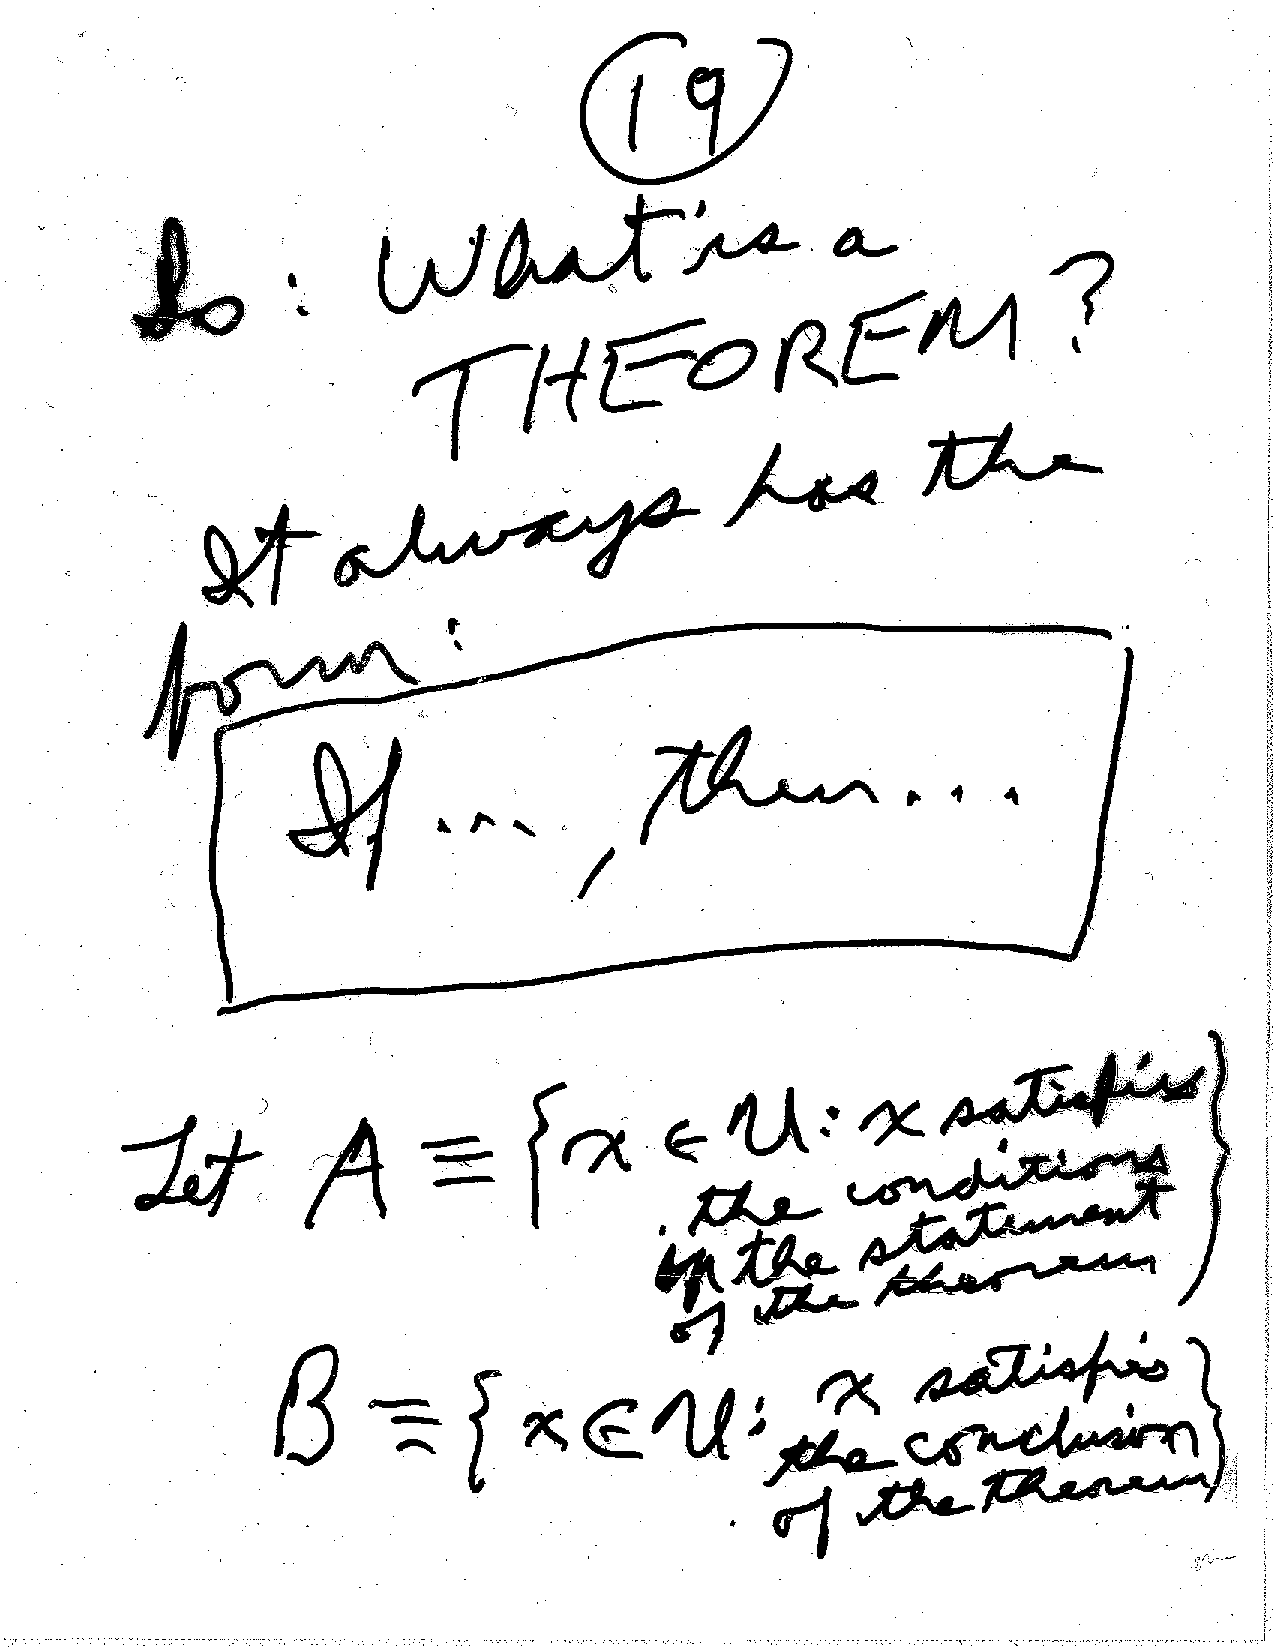
\includegraphics[scale=.5]{Pages/ST_19}

\newpage

\noindent Hence, this theorem can be nested as nothing other than $A \subseteq B $.
\\ \indent Hence, a proof is just a logical demonstration:
\\ \indent For each $x \in A$, in fact $x \in B$ also.

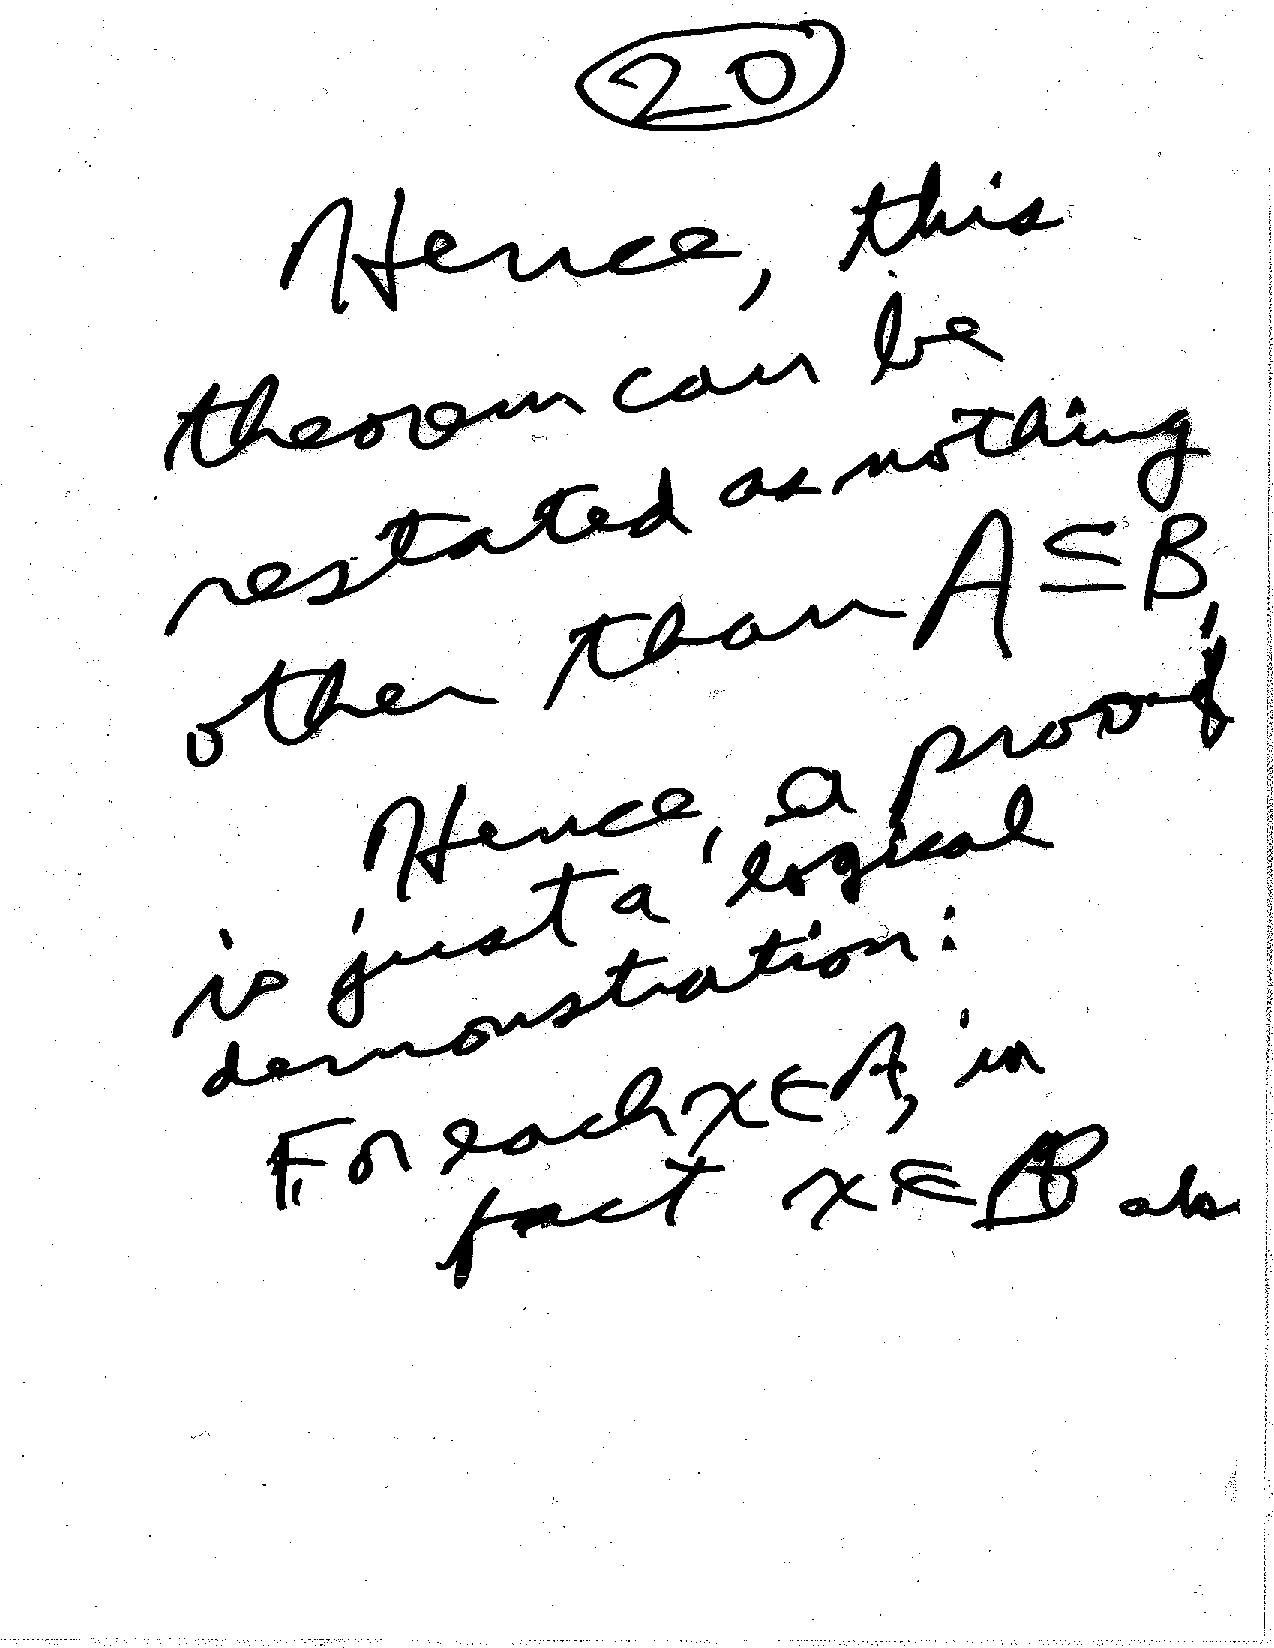
\includegraphics[scale=.5]{Pages/ST_20}

\newpage

\noindent It is beyond the scope of this course to formalize how the statement $A \subseteq B$ may be proved. However, to illustrate what is required, it is sufficient to show:
\vspace{2mm}
\\ For each $x \in A$, there exists sets 
$$ D_{x, 1} \subseteq D_{x, 2} \subseteq D_{x, 3} \subseteq \cdots $$
\\ such that $x \in D_{x, 1}$ \underline{and}
$$ \bigcup_{j=1}^{\infty} D_{x, j} \subseteq B$$

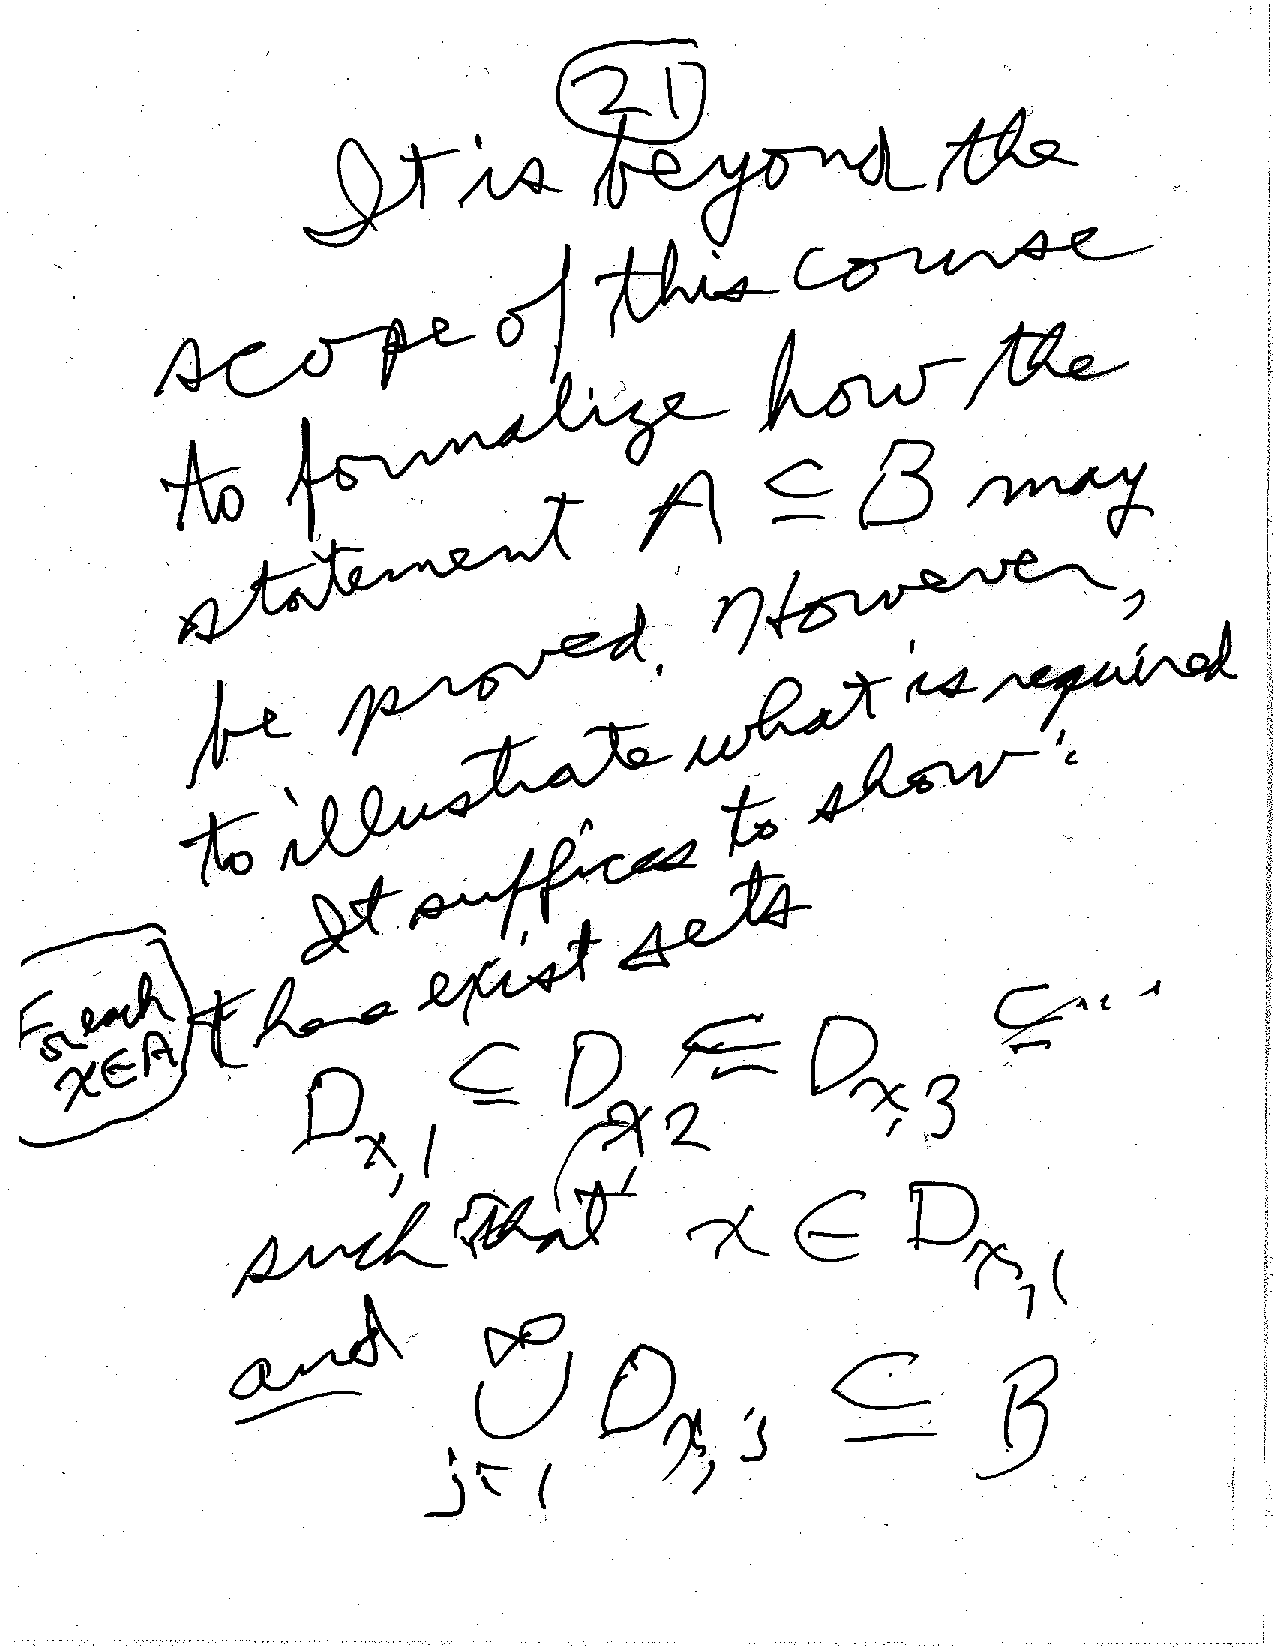
\includegraphics[scale=.5]{Pages/ST_21}







 
%Maady: IS33 - IS42

\section{Metric Spaces Part 1}

%Travis: M1 - M5

%Jerome: M6- M10



\section{Metric Spaces Part 2}


%Bryant: M1-M7

%Reshma: M8-M14

%Ethan: M15-M21





\end{document}